\documentclass[11pt,a4paper,twoside,openany]{article}
\usepackage{amsmath,amsbsy,a4wide,amssymb,amsthm}
\usepackage{color,graphics}
\usepackage{natbib}
\usepackage{array}
\usepackage{cancel}
\usepackage{psfrag}
\usepackage{times}
\usepackage{lscape}
\usepackage{rotating}
\usepackage{longtable}	%for tables spanning multiple pages
\usepackage{supertabular}
\usepackage{multirow}
\usepackage[toc,page]{appendix}
\usepackage{thumbpdf}   %PDF specific
\usepackage[pdftex,
        colorlinks=true,
        urlcolor=rltblue,       % \href{...}{...} external (URL)
        filecolor=rltblack,     % \href{...} local file
        linkcolor=rltblack,       %\ref{...} and \pageref{...}
        citecolor=rltblack,
        pdftitle={A Gmsh tutorial},
        pdfauthor={AMCG},
        pdfsubject={},
        pdfkeywords={},
        pdfpagemode=None,
        bookmarksopen=true,
        plainpages=false]{hyperref}
\usepackage{color}
\definecolor{rltblack}{rgb}{0,0,0}
\definecolor{rltred}{rgb}{0.75,0,0}
\definecolor{rltgreen}{rgb}{0,0.5,0}
\definecolor{rltblue}{rgb}{0,0,1}
\usepackage[]{caption}
\renewcommand{\captionfont}{\linespread{1.5}\small\itshape}
\renewcommand{\captionlabelfont}{\linespread{1.1}\small\itshape\bfseries}
\setlength{\captionmargin}{20pt}
\usepackage{pdfpages}
\usepackage{subfig}
\usepackage{listings}
\lstset{basicstyle=\ttfamily\small,numbers=none,stepnumber=1,numberstyle=\tiny,commentstyle=\color{rltblue},keywordstyle=\color{rltred}}
\usepackage{eso-pic}

\def \ie{{\it\frenchspacing i.e.\ }}
\def \eg{{\it\frenchspacing e.g.\ }}
\def \cf{{\it\frenchspacing cf.\ }}
\def \etc{{\it\frenchspacing etc.\ }}
\def \viz{{\it\frenchspacing viz.\ }}
\def \etal{{\it\frenchspacing et al.\ }}

%% Header Style
\usepackage{fancyhdr}
\pagestyle{fancy}

\renewcommand{\sectionmark}[1]{\markright{\footnotesize{\thesection.\ #1}}{}}
\renewcommand{\leftmark}{A Gmsh tutorial}
\fancyhead[LE,RO]{\thepage}
\fancyhead[RE]{\leftmark}
\fancyhead[LO]{\rightmark}
\fancyfoot[LE,RO]{\footnotesize{\href{http://amcg-www.ese.ic.ac.uk/index.php?title=Main_Page}{AMCG}}}
\cfoot{} %cancel out default printing of page number at bottom-centre of the page
\renewcommand{\headrulewidth}{0.4pt}
\renewcommand{\footrulewidth}{0.0pt}
\setlength{\headheight}{7mm}
\setlength{\headwidth}{150mm}

%Boxed align equations
\newenvironment{boxalign}
{\fbox{ \addtolength{\linewidth}{-2\fboxsep} \addtolength{\linewidth}{-2\fboxrule} \begin{minipage}{\linewidth} \begin{align} }
{\end{align} \end{minipage} } }

\newcommand{\NSeq}{Navier-Stokes equations\ }
% differential operator
\newcommand{\dif}{\ensuremath{~\mathrm{d}}}
% generic partial derivative
\newcommand{\pderiv}[2]{\ensuremath{\frac{\partial #1}{\partial #2}}}
%spatial partial derivative
\newcommand{\pdx}[2]{\pderiv{#1}{x_{#2}}}
%temporal partial derivative
\newcommand{\pdt}[1]{\pderiv{#1}{t}}
%generic 2nd derivative
\newcommand{\cpderiv}[3]{\ensuremath{\frac{\partial^2 #1}{\partial #2
	\partial #3}}}
%laplacian
%\newcommand{\lapl}[2]{\ensuremath{\frac{\partial^2 #1}{{\partial x_{#2}}^2}}}
\newcommand{\lapl}[2]{\cderiv{^2 #1} {x_{#2}} {x_{#2}} }
%Bold-face-italic tensor  and vector notation
\newcommand{\tnsr}[1]{\mbox{\overline{\overline{$#1$}}}}
\newcommand{\vctr}[1]{\ensuremath{\overrightarrow{#1}}}
%Sans-serif matrix notation
\newcommand{\matrx}[1]{\ensuremath{\mathsf{#1}}}

%Filtered notation: overbar
\newcommand{\filt}[1]{\ensuremath{\overline{#1}}}
%Single-variable Integrals
\newcommand{\myint}[2]{\ensuremath{\int_{#1}{#2} \mbox{ \bf{d}} {#1}}}
\newcommand{\myintlu}[4]{\ensuremath{\int_{#1}^{#2}{#3} \mbox{ \bf{d}} {#4}}}

\begin{document}

\baselineskip=18pt

\begin{titlepage}
\setlength{\hoffset}{0pt}
\setlength{\voffset}{0pt}
\setlength{\oddsidemargin}{-1in}
\setlength{\topmargin}{-1.5in}
\setlength{\textwidth}{\paperwidth}

\begin{minipage}[t]{2.5in}
\baselineskip=10pt
{\footnotesize
Fluidity training documentation\\
Applied Modelling and Computation Group (AMCG)\\
\url{http://amcg-www.ese.ic.ac.uk/}\\
Imperial College London}
\end{minipage}\\[40mm]

\begin{minipage}{\textwidth}
\begin{center}
\huge A Gmsh tutorial\\[10mm]
\normalsize A. Avdis and S.L.Mouradian\\
AMCG
\end{center}
\end{minipage}
\\[10mm]
\begin{minipage}{0.1\paperwidth}
\hfill
\end{minipage}
\begin{minipage}{0.8\paperwidth}
 \begin{center}
 \begin{minipage}[t]{3.2in}
 \section*{Summary}\small
This document is a tutorial on the Gmsh mesh generator. It is aimed towards complete beginners; only
some basic knowledge of the Linux terminal and a text editor is assumed. We first define what a mesh
is and then introduce the reader to the basics of the Gmsh graphical user interface. A basic,
two-dimensional, geometry is then constructed within Gmsh and a mesh is constructed. A more
complicated three-dimensional annulus is also constructed and meshed, demonstrating some
more advanced features of Gmsh.

Having mastered the basic usage of the graphical user interface, users are introduced to generating
simple meshes on the sphere. Finally, other tutorials and methds that show how to produce
meshes in realistic domains are briefly introduced in the last section.
%Knowledge is further built to produce meshes of realistic domains
%of the oceans to include boundaries extracted from a high resolution shorelines database.
   %Summary goes here
 \end{minipage}\hfill
 \begin{minipage}[t]{3in}{\footnotesize{\tableofcontents}}\end{minipage}\\[10pt]
 \end{center}
\end{minipage}
\AddToShipoutPicture*{%
  \AtPageLowerLeft{%
        \begin{minipage}{\paperwidth}
          \hfill
          \scalebox{0.05}{
\includegraphics{Logo_white.png}}\\[30pt]
        \end{minipage} %
    } %
  }%
\end{titlepage}
\thispagestyle{empty}
\begin{center}
%Do not copy or reproduce without the explicit consent of all authors.\\[40mm]
This document was compiled on \today\\
%url to the latest version:\\
%\url{http://amcg.ese.ic.ac.uk/files/gmsh_tutorial.pdf}\\
%fluidity licence statement?\\
%QR to documet url? (ok, that one is perhaps too gimicky)
\end{center}
\pagebreak

\setlength{\textwidth}{390pt}
\setlength{\textheight}{592pt}
\setlength{\topmargin}{-0.5in}
\setlength{\headsep}{10mm}
\setlength{\textheight}{240mm}
\setlength{\oddsidemargin}{4mm}
\setlength{\evensidemargin}{-4.mm}
\pagenumbering{arabic}

\section{Introduction}
\label{sect:introduction}

\subsection{What is a mesh?}
\label{ssect:mesh_definition}
\par
A mesh can be qualitatively thought of as the tessellation of a domain $\Omega$ into a set of
non-overlapping subdomains $\omega_i$:
\begin{align}
\Omega &= \cup \left\{ \omega_i \left| i=1,2,\ldots ele \right. \right\} \nonumber \\
\label{eqn:tessalation_definition} \\
0 &= \cap \left\{ \omega_i \left| i=1,2,\ldots ele \right. \right\} \nonumber
\end{align}
where $ele$ is the number of elements in the tessellation. Figure \ref{fig:1d_2d_mesh_examples} shows
meshes on one-dimensional and two-dimensional domains. The extension to three-dimensional domains
is clear. Whatever the dimensionality of the domain, it is evident from figure \ref{fig:1d_2d_mesh_examples} that the mesh can be constructed
by first distributing a set of nodes throughout the domain, and then connect the nodes, so as to obtain
a set of non--overlapping elements. Therefore, in order to define a mesh, one needs to define node locations,
as well as element topology consistent to equations \eqref{eqn:tessalation_definition}.
\begin{figure}[htbp]
 \centering
  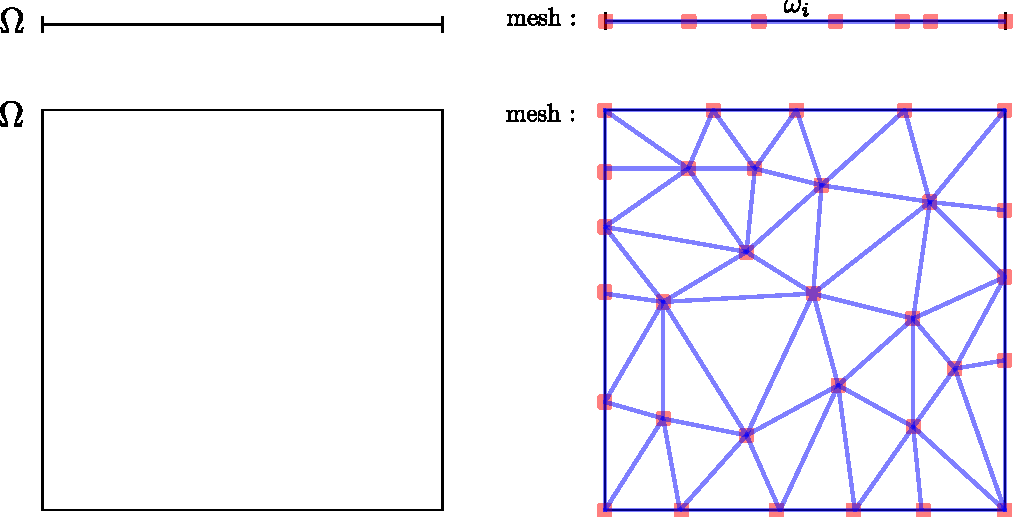
\includegraphics[width=1.0\textwidth]{../figures/1d_2d_mesh_examples}
  \caption{Examples of meshes in one-dimensional and two-dimensional domains.}
  \label{fig:1d_2d_mesh_examples}
\end{figure}

\subsection{What is Gmsh?}
\label{sect:Gmsh}
\par
It is the task of a \emph{mesh generator} to create node locations and element topology so as to create high quality meshes. Gmsh is a \emph{``3D finite element grid generator with a build-in CAD engine and post-processor. Its design goal is to provide a fast, light and user-friendly meshing tool with parametric input and advanced visualisation capabilities.''}\footnote{from \url{http://www.geuz.org/gmsh/}}. Furthermore, Gmsh can be used as a 1--, 2-- and 3-- dimensional mesh generator for use with Fluidity.
\par
Gmsh is developed by~\cite{Geuzaine_Remacle_2009} and distributed under the terms of the GNU General Public License. Executables for Linux, Windows and Mac OS can be downloaded from \url{http://www.geuz.org/gmsh/} as well as the source code. In Linux distributions where the Advanced Package Tool (APT) is available (such as Ubuntu), typing \lstinline{sudo apt-get install gmsh} in a terminal will probably install Gmsh on your system. The rest of this tutorial assumes that Gmsh is run on Linux. 
\par
Gmsh's architecture is centred around four modules:
\begin{enumerate}
  \item Geometry
  \item Mesh
  \item Solver
  \item Post-processing
\end{enumerate}
In this tutorial we will only use the Geometry and Mesh modules. As suggested by their names the geometry
module is used to define geometrical objects, such as points, lines, surfaces and volumes, while the
mesh module is used to create meshes (nodes and element topology).

\subsubsection{Starting Gmsh}
\begin{figure}[htbp]
 \centering
  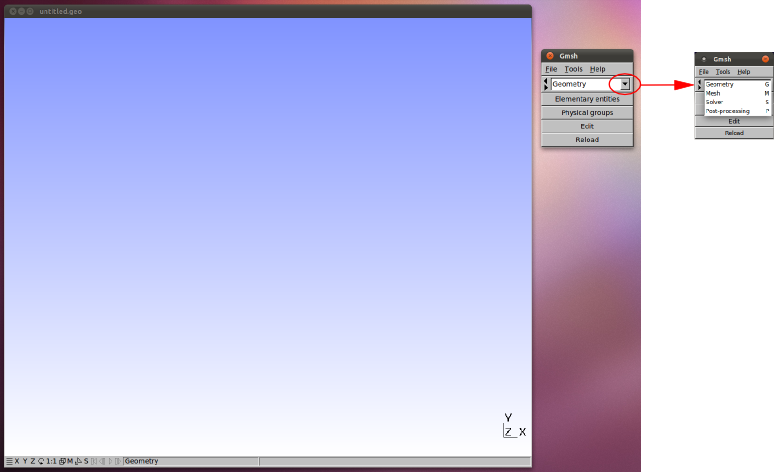
\includegraphics[width=1.0\textwidth]{../figures/gmsh_startup_and_modules.png}
  \caption{Left panel: The Gmsh windows after startup. The larger window is termed the Graphic window
           and the smaller window is termed the Menu window.}
  \label{fig:gmsh_startup_and_modules}
\end{figure}
Gmsh can be started by issuing the following command at the Terminal:
\begin{lstlisting}
gmsh mymesh.geo
\end{lstlisting}
where \lstinline{mymesh.geo} is the name of the newly created file to store your geometry. If a file is
not named, an \lstinline{untitled.geo} file will be created. For this tutorial, it is best practice to
name your files and avoid using an ``untitled'' document. As the Gmsh user interacts with the GUI,
her/his actions are stored in the \lstinline{.geo} file, in the form of script commands. One can modify
the script with any text editor. Once Gmsh is opened, you will be presented with the Gmsh
\emph{menu} and \emph{graphic} windows, as illustrated in
figure~\ref{fig:gmsh_startup_and_modules}.

\subsubsection{Basic interaction with the Graphical User Interface}
\label{ssect:basic_interaction_gmsh_gui}

Once Gmsh is opened, you will be presented with the Gmsh \emph{menu} and \emph{graphic} windows, as
illustrated in figure~\ref{fig:gmsh_startup_and_modules}.
The \emph{menu window} allows the user to access features of the Gmsh graphical user interface, while
the \emph{graphic window} displays the defined points, lines and any other geometrical objects. The
modular architecture of Gmsh is reflected in the menu window; clicking on the down-pointing arrow next
to ``Geometry'' produces a drop-down menu (as shown in figure \ref{fig:gmsh_startup_and_modules}),
allowing the user to select any of the four modules listed in section \ref{sect:Gmsh}.
\begin{figure}[htbp!]
 \centering
  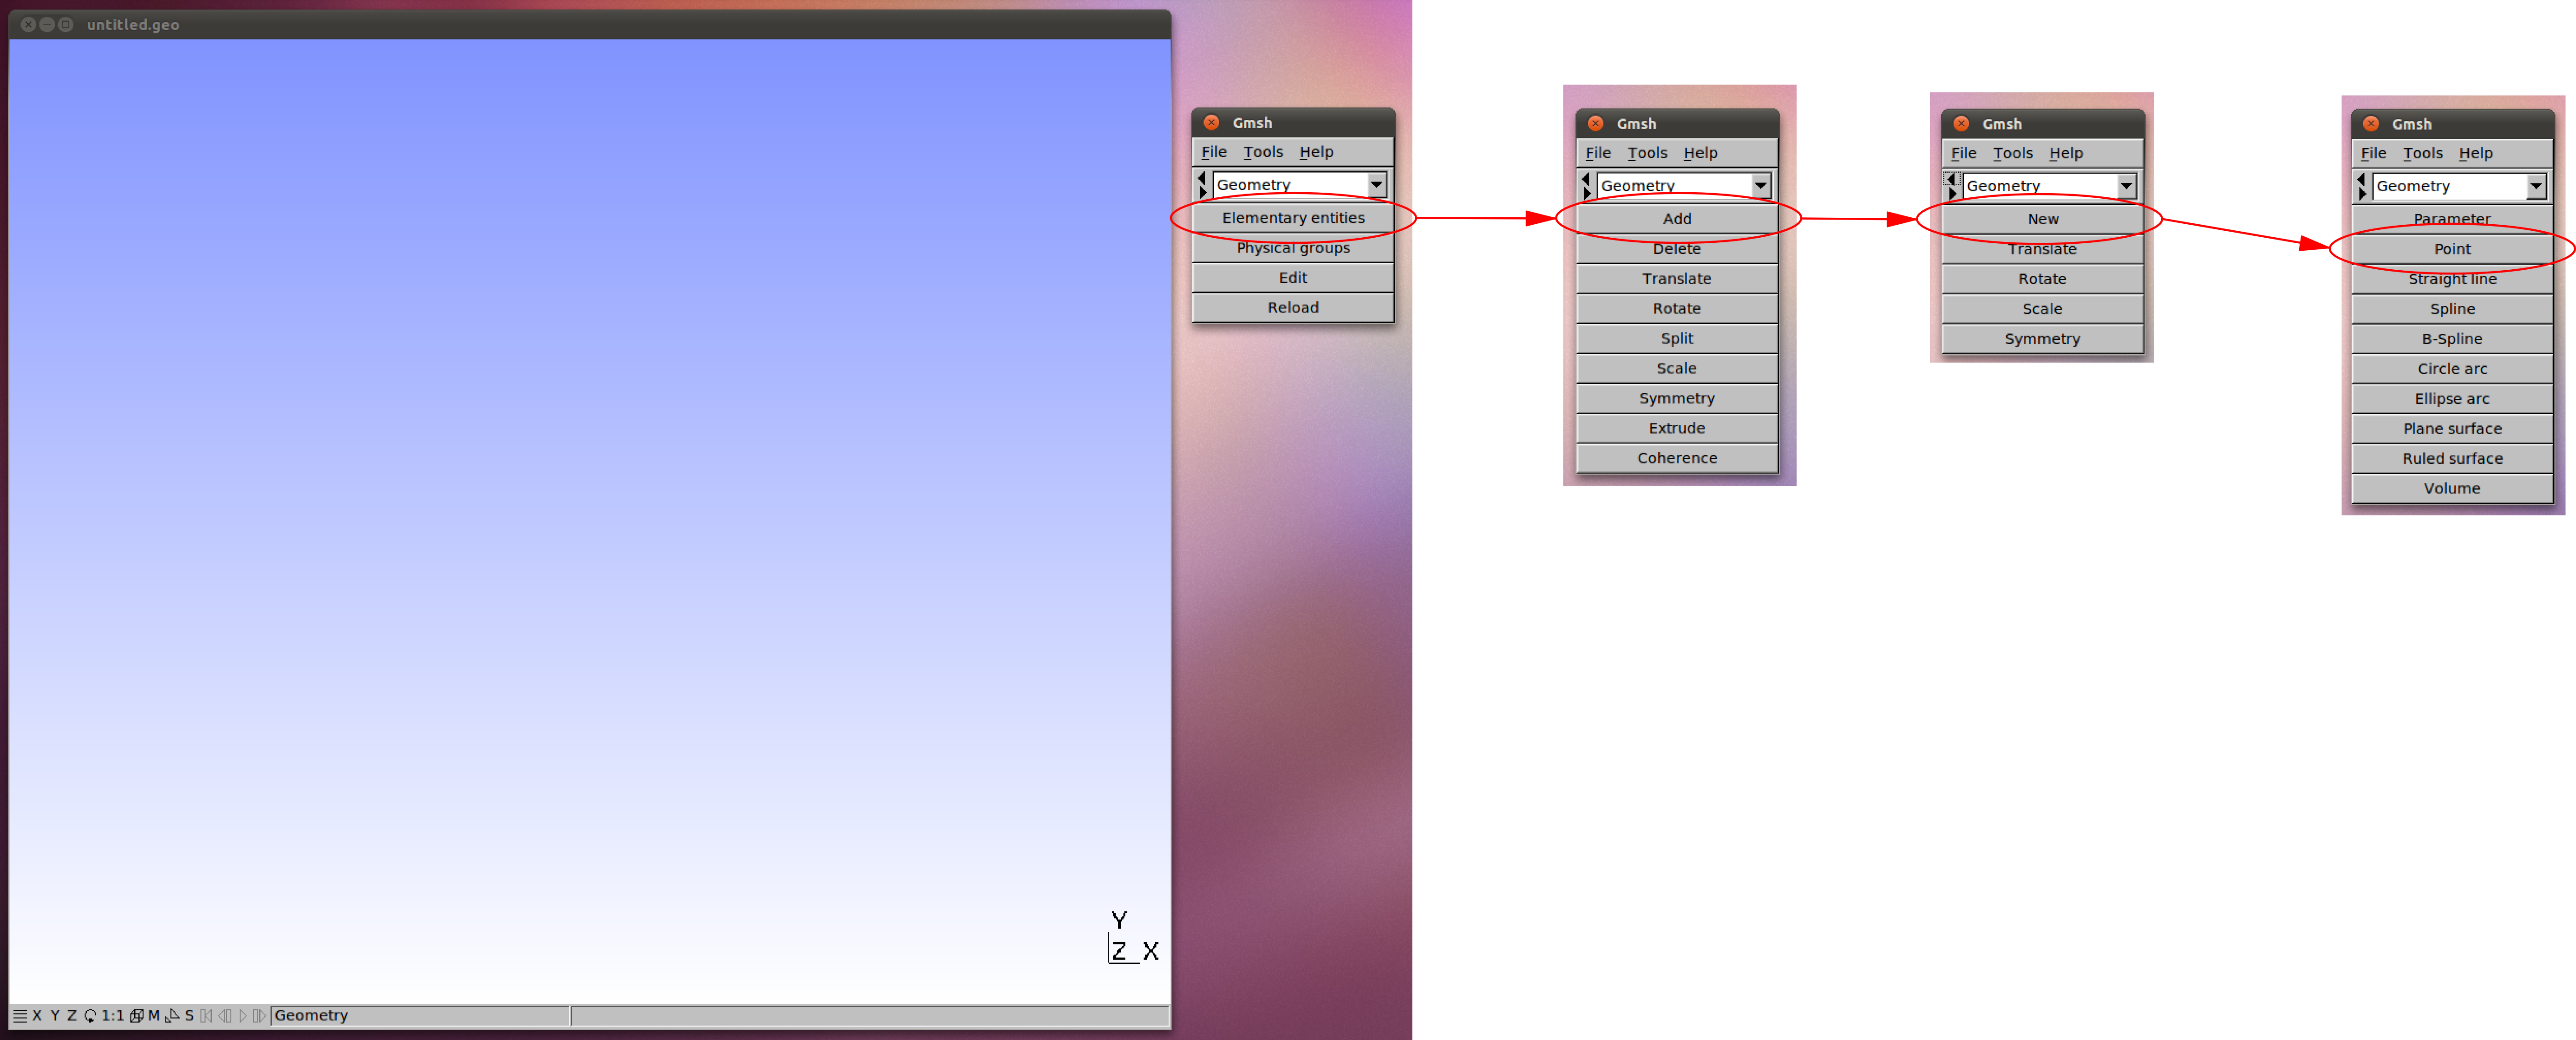
\includegraphics[width=1.0\textwidth]{../figures/getting_started.png}
  \caption{Basic interaction with the GMSH GUI}
  \label{fig:basic_interaction}
\end{figure}
Familiarise yourself with the Gmsh menu window, by navigating to a mode that allows you to add a point.
Try the following for yourself to get comfortable navigating the menu and understand the notation
provided above, which will be used through this tutorial to point you to specific features of Gmsh.
\begin{enumerate}
  \item Click on \lstinline{Geometry (G) > Elementary entities > Add > New > Point}, as indicated in
        figure \ref{fig:basic_interaction}. After clicking on ``Point'' in the menu window the 
        ``Contextual Geometry Definitions'' window will appear and a message appears at the top
        of the Graphic window, as shown in figure \ref{fig:creating_a_point}.
  \item Close the Contextual Geometry Definitions window and press ``q'' to abort the command.
  \item You may use the keyboard buttons $G$, $M$, $S$ and $P$ to get to the top-level of the
        Geometry, Mesh, Solvers and Post-processing modules respectively. Press $G$ to return to
        the top-level of the Geometry module. Try switching to the Mesh module and then back to
        the Geometry module.
\end{enumerate}

\begin{figure}[htbp]
 \centering
  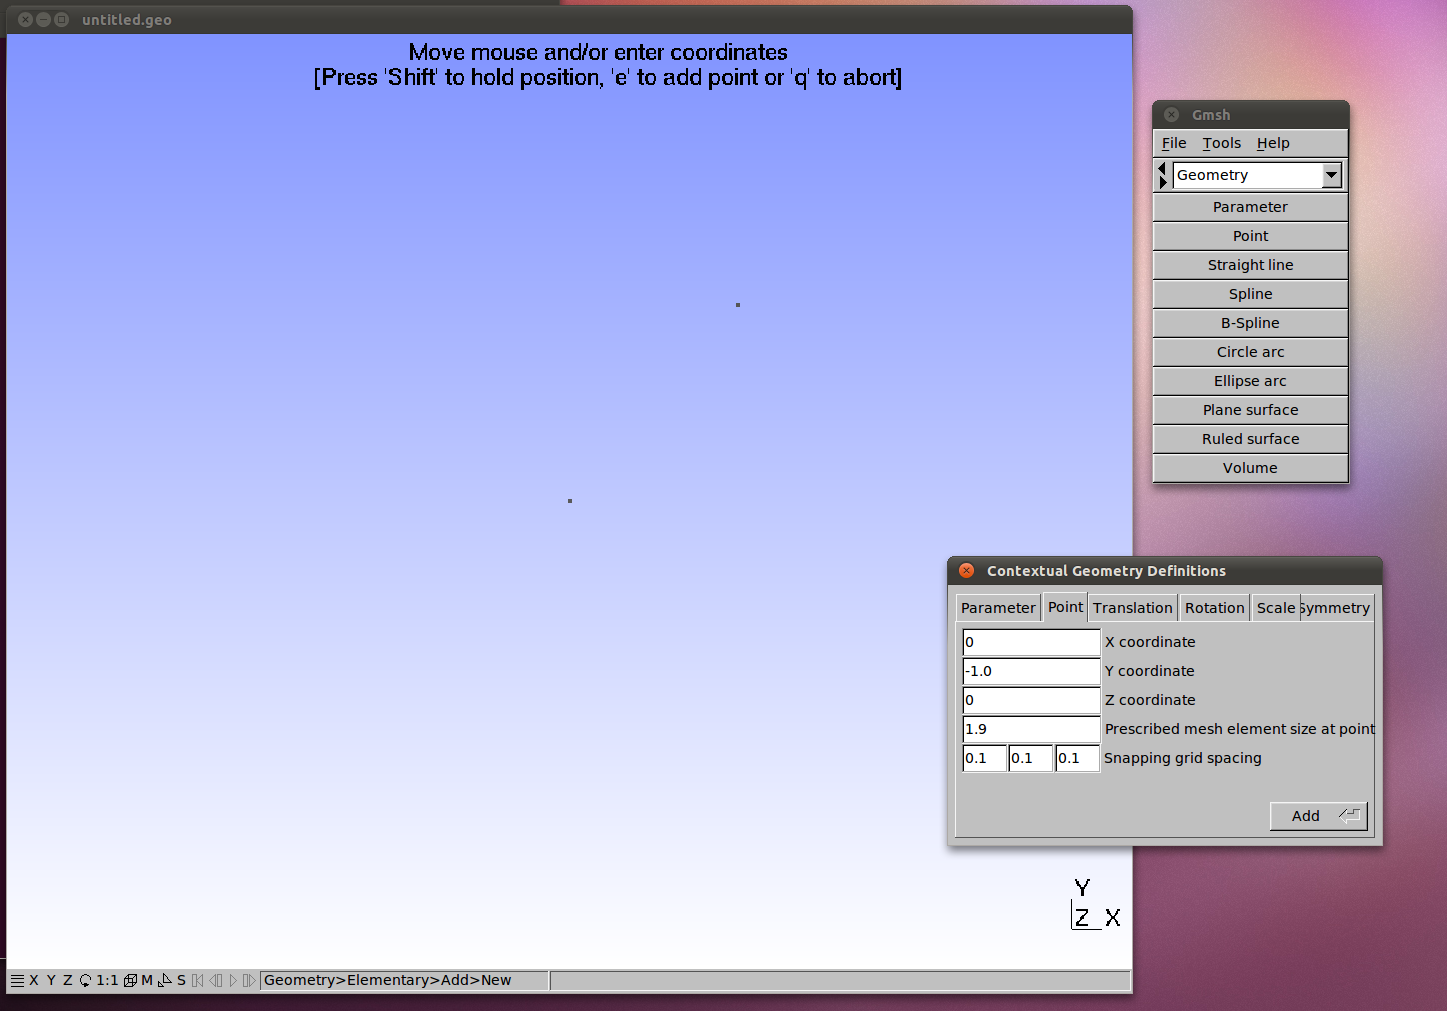
\includegraphics[width=0.8\textwidth]{../figures/shot5.png}
  \caption{Creating a point.}
  \label{fig:creating_a_point}
\end{figure}

We will now open an existing geometry and learn to navigate by panning, zooming and rotating. To obtain the geometry, please download the file at:
\begin{lstlisting}
http://amcg.ese.ic.ac.uk/download/annulus.geo
\end{lstlisting}
and open it by issuing the following at the command line:
\begin{lstlisting}
gmsh annulus.geo
\end{lstlisting}

Once open, you should see the geometry illustrated in figure~\ref{fig:annulus1}. On the bottom-left of the graphic window,
you will see various tools available to manage the view.
The $X$, $Y$ and $Z$ buttons align the corresponding axis perpendicular to the screen. Try selecting the
$X$ view, as in figure~\ref{fig:annulus2}. Both these views are not particularly useful in understanding
the annulus domain. Try to rotate the geometry by left-clicking and holding on the screen, then moving the mouse pointer.
Try to get the geometry as illustrated in figure~\ref{fig:annulus3}. You can pan the geometry by right-clicking and moving the mouse. To zoom, simply use the scroll. Alternatively, you may hold the middle-button and move the mouse. Make sure you familiarise yourself with manipulating the orientation of your domain, as this will be useful later on.

\begin{figure}[htbp!]
  \centering
  \subfloat[Default view]{\label{fig:annulus1}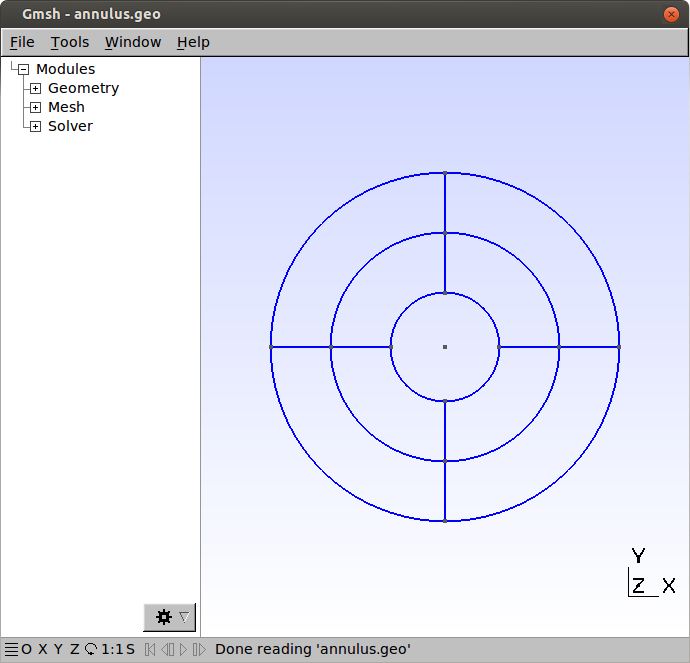
\includegraphics[width=0.45\textwidth]{../figures/annulus1}}
  \subfloat[x--axis perpendicular to screen]{\label{fig:annulus2}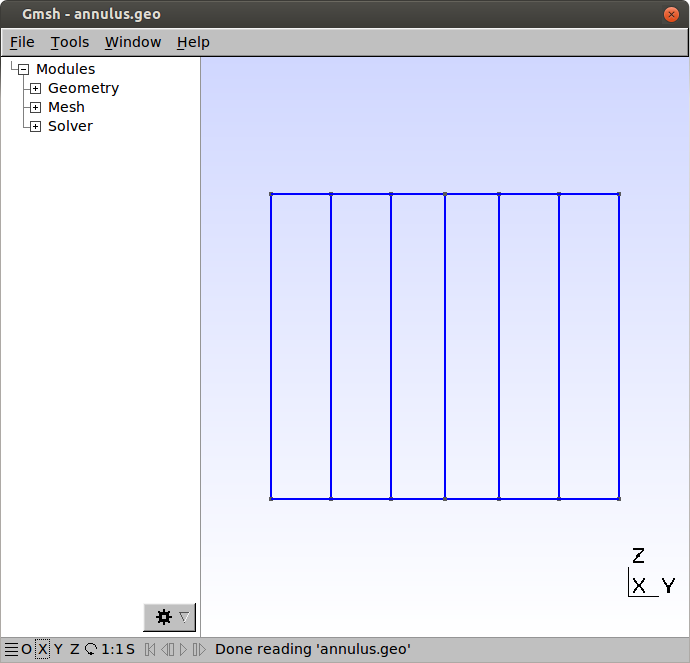
\includegraphics[width=0.45\textwidth]{../figures/annulus2}}\\
  \subfloat[Rotated view]{\label{fig:annulus3}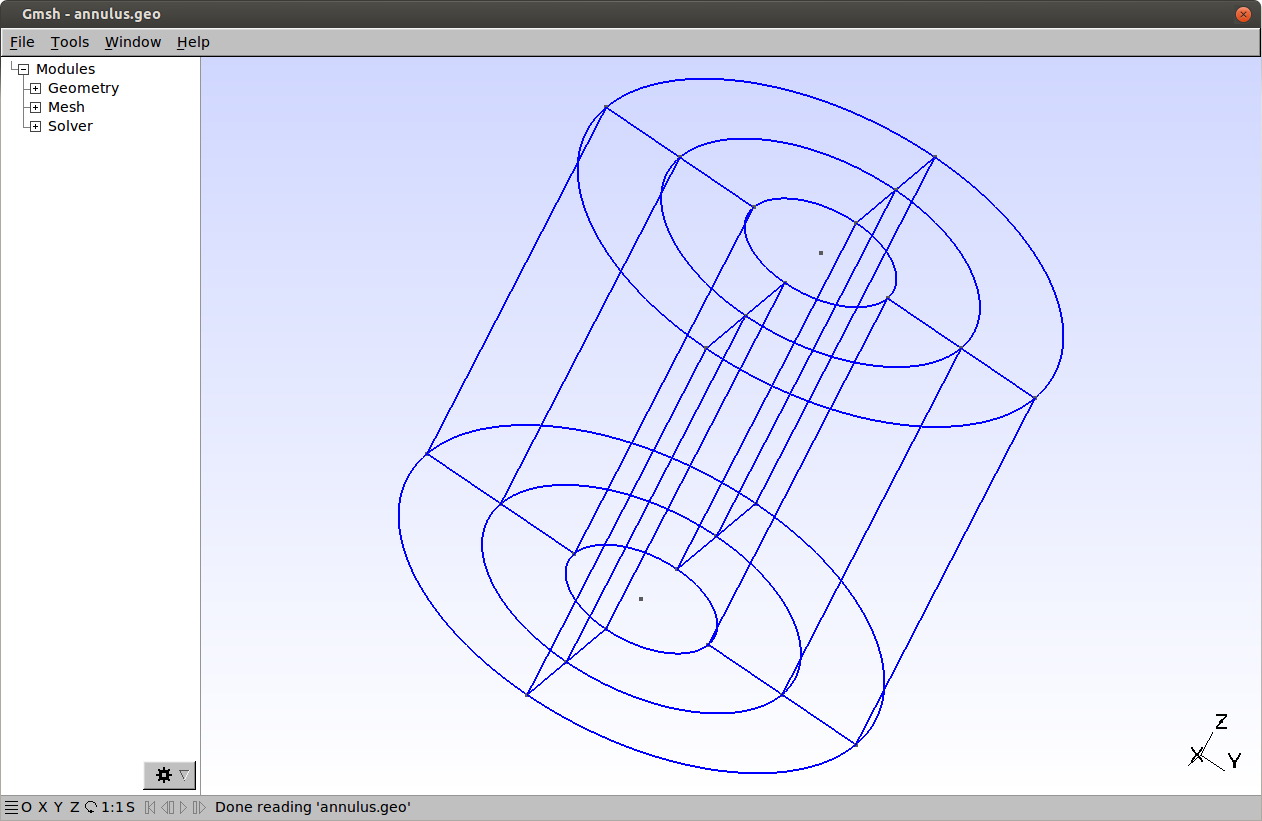
\includegraphics[width=0.45\textwidth]{../figures/annulus3}}
  \subfloat[Meshed and zoomed]{\label{fig:annulus4}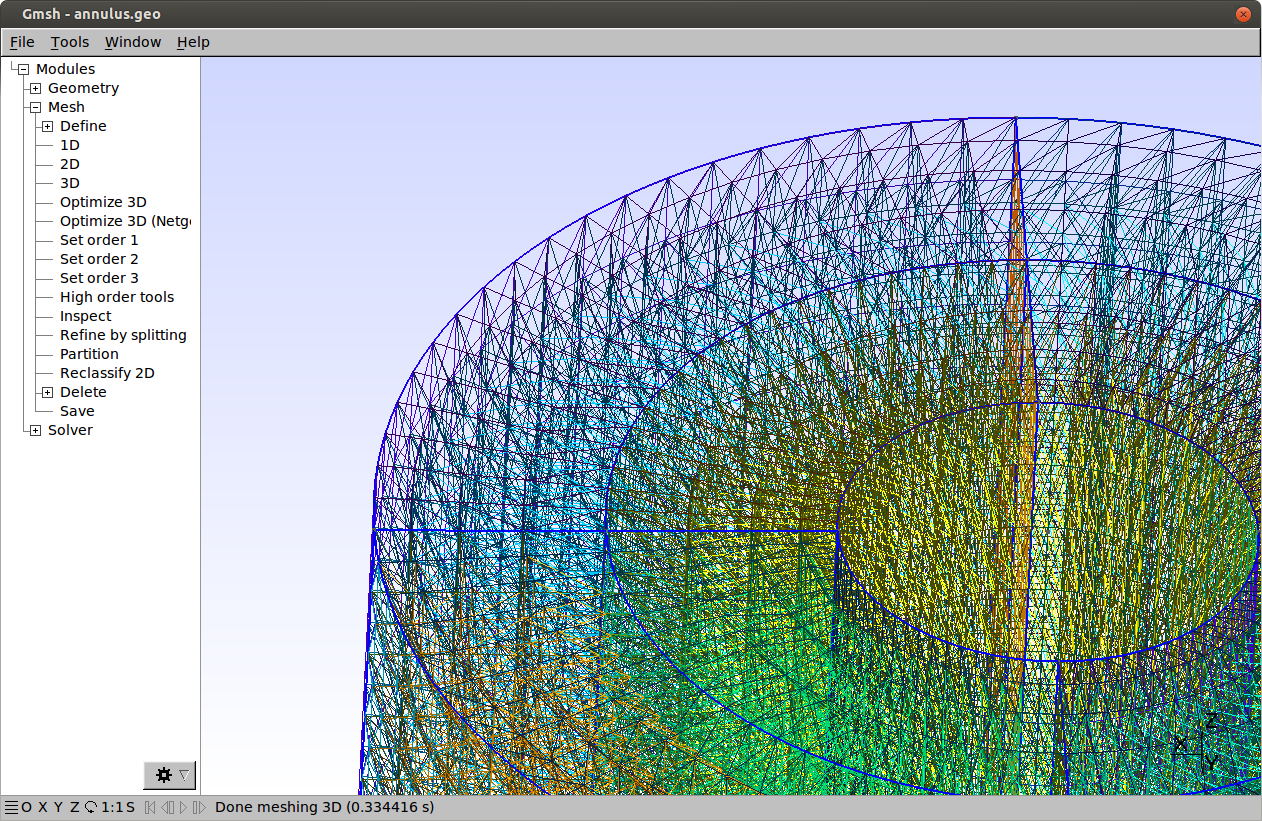
\includegraphics[width=0.45\textwidth]{../figures/annulus4}}
  \caption{Panning, zooming, rotating and manipulating the Gmsh graphic window.}
  \label{fig:animals}
\end{figure}
\par
As no meshing tutorial can be complete without a mesh, we end by meshing the geometry. To generate a mesh of this domain, go to:
\begin{lstlisting}
Mesh (M) > 3D
\end{lstlisting}
This can be done by pressing your keyboard's $M$ key, and then selecting $3D$ to mesh the three--dimensional domain. Figure \ref{fig:annulus4} shows a view of the meshed annulus.



\section{A two dimensional example}
\label{sect:two_dimensional_example}
\par
In this example we aim to create a mesh in a rectangle, as shown in figure
\ref{fig:shot16}.
%\begin{figure}[htbp]
%\centering
%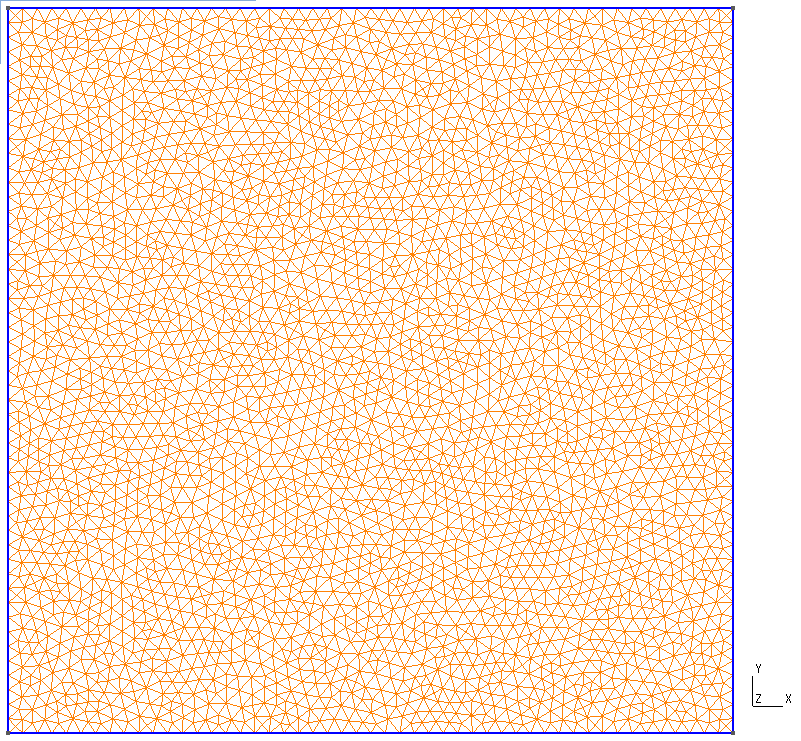
\includegraphics[width=1.0\textwidth]{../figures/2d-example-mesh.png}
%\caption{Mesh on the rectangle}
%\label{fig:2d-example-mesh}
%\end{figure}
The following steps will be taken:
\begin{enumerate}
  \item Set up the geometry. The graphical user interface of Gmsh is used to carry out the following
           steps:
  \begin{enumerate}
    \item Create the two points on the left-hand side of the rectangle.
    \item Connect the two points with a line
    \item Extrude the line to form the rectangle.
  \end{enumerate}
  \item Define physical groups. Defining physical groups results into numerical ID's being assigned to
           each group. Fluidity uses these ID's to apply boundary conditions.
  \item Customise the geometry. A subset of the Gmsh scripting language is introduced and modifications
           will be made to the geometry script.
  \item Produce a mesh.
\end{enumerate}
The following sections go through the above steps, in great detail.

\subsection{Setting up the geometry}
\label{ssect:setting_up_geometry}
\par
\par
Run gmsh on the command line, storing the geometry in \lstinline{channel.geo}:
\begin{lstlisting}
gmsh channel.geo
\end{lstlisting}
\par
Create the points at the left-hand-side of the rectangle:
\begin{enumerate}
  \item Go to the top-most level of the Geometry module in the menu window.
  \item On the menu window click on \lstinline{Elementary entities > Add > New > Point} , see
        figure \ref{fig:basic_interaction}. The ``Contextual Geometry Definitions'' window will
        appear at the point tab, as shown in figure \ref{fig:creating_a_point}.
        Note that  moving the cursor over the graphic window will cause the coordinates shown in
        the Contextual Geometry Definitions window to change. While the user is allowed to specify
        points using this interactive \& graphical interface, we will directly enter the point
        coordinates on the Contextual Geometry Definitions window. Doing so allows for more accurate
        control of the point coordinates.
  \item Add a point at $(x,y,z)=(0,-1,0)$, with a characteristic mesh element size of $1.9$: Modify the
        parameters in the Contextual Geometry Definitions window, to match those shown in
        figure \ref{fig:creating_a_point} and click on ``Apply'' (on the same window). Be careful not
        to move the cursor over the graphic window, as it will change your coordinates.
  \item Add another point at $(0,1,0)$
  \item Close the Contextual Geometry Definitions window.
\end{enumerate}
\par
Create a line representing the left-hand edge of the rectangle:
\begin{enumerate}
  \item Click on \lstinline{Geometry (G) > Elementary entities > Add > New > Straight line}
  \item Choose the starting point of the line segment on the graphic window. Note that the
        starting point should now be coloured red. If not, try selecting it again.
  \item Choose the ending point of the line segment. If the point selection is successful,
        the straight line segment should appear in the graphic window, and you should have
        something similar to the left-most panel in figure \ref{fig:gmsh_extrusion}.
  \item Press ``q'' on your keyboard.
\end{enumerate}
\begin{figure}[htbp]
 \centering
  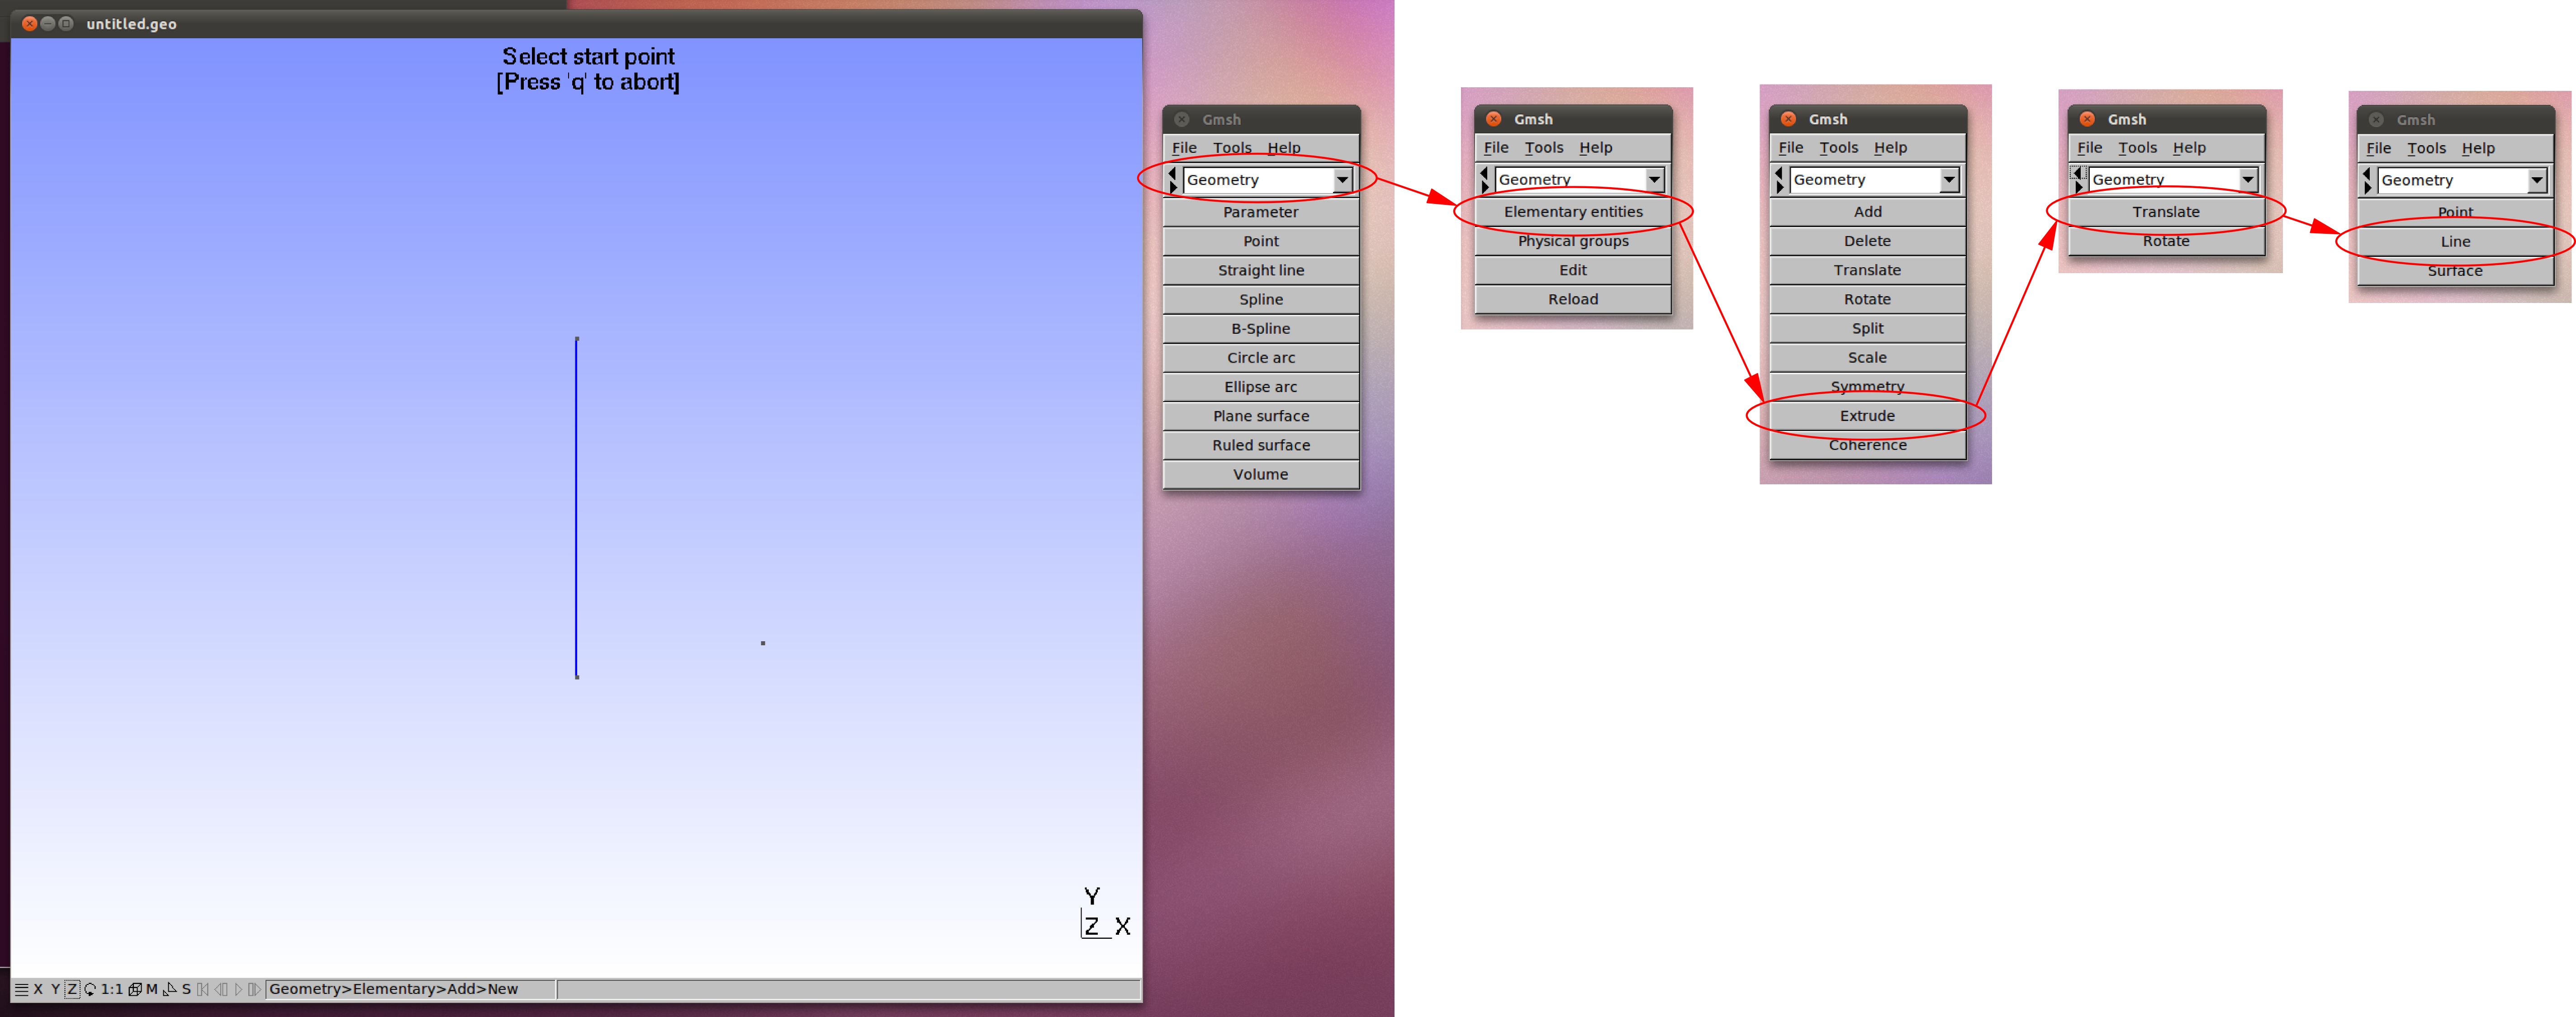
\includegraphics[width=1.0\textwidth]{../figures/navigating_to_extrusion.png}
  \caption{Directing Gmsh to extrusion.}
  \label{fig:gmsh_extrusion}
\end{figure}
\par
Note that one could simply create all four points at the rectangle vertices and then simply draw the
lines to from the rectangle sides. However, extrusions  are used below as it demonstrates more features
of Gmsh and it facilitates the creation of a structured mesh:
\begin{enumerate}
  \item Go to the top-most level of the Geometry module in the menu window.
  \item Click on \lstinline{Elementary entities > Extrude > Translate > Line},
        as indicated in figure \ref{fig:gmsh_extrusion}. The Contextual Geometry Definitions window will
        appear, set to the Translation tab, as shown in the left panel of figure \ref{fig:extrusion}
  \item Modify the parameters in the Contextual Geometry Definitions window to specify an extrusion
        along the $x$-direction of $10$ length-units, as shown in the left panel of
        figure \ref{fig:extrusion}.
  \item Click on the line we previously drew on the graphical window, it should be highlighted in red,
        as shown in the left panel of figure \ref{fig:extrusion}.
  \item Press the key ``e'' on your keyboard, a rectangle should appear in the graphical window, as shown
        in the right panel of figure \ref{fig:extrusion}.
  \item Close the Contextual Geometry Definitions window.
\end{enumerate}
\begin{figure}[htbp]
 \centering
  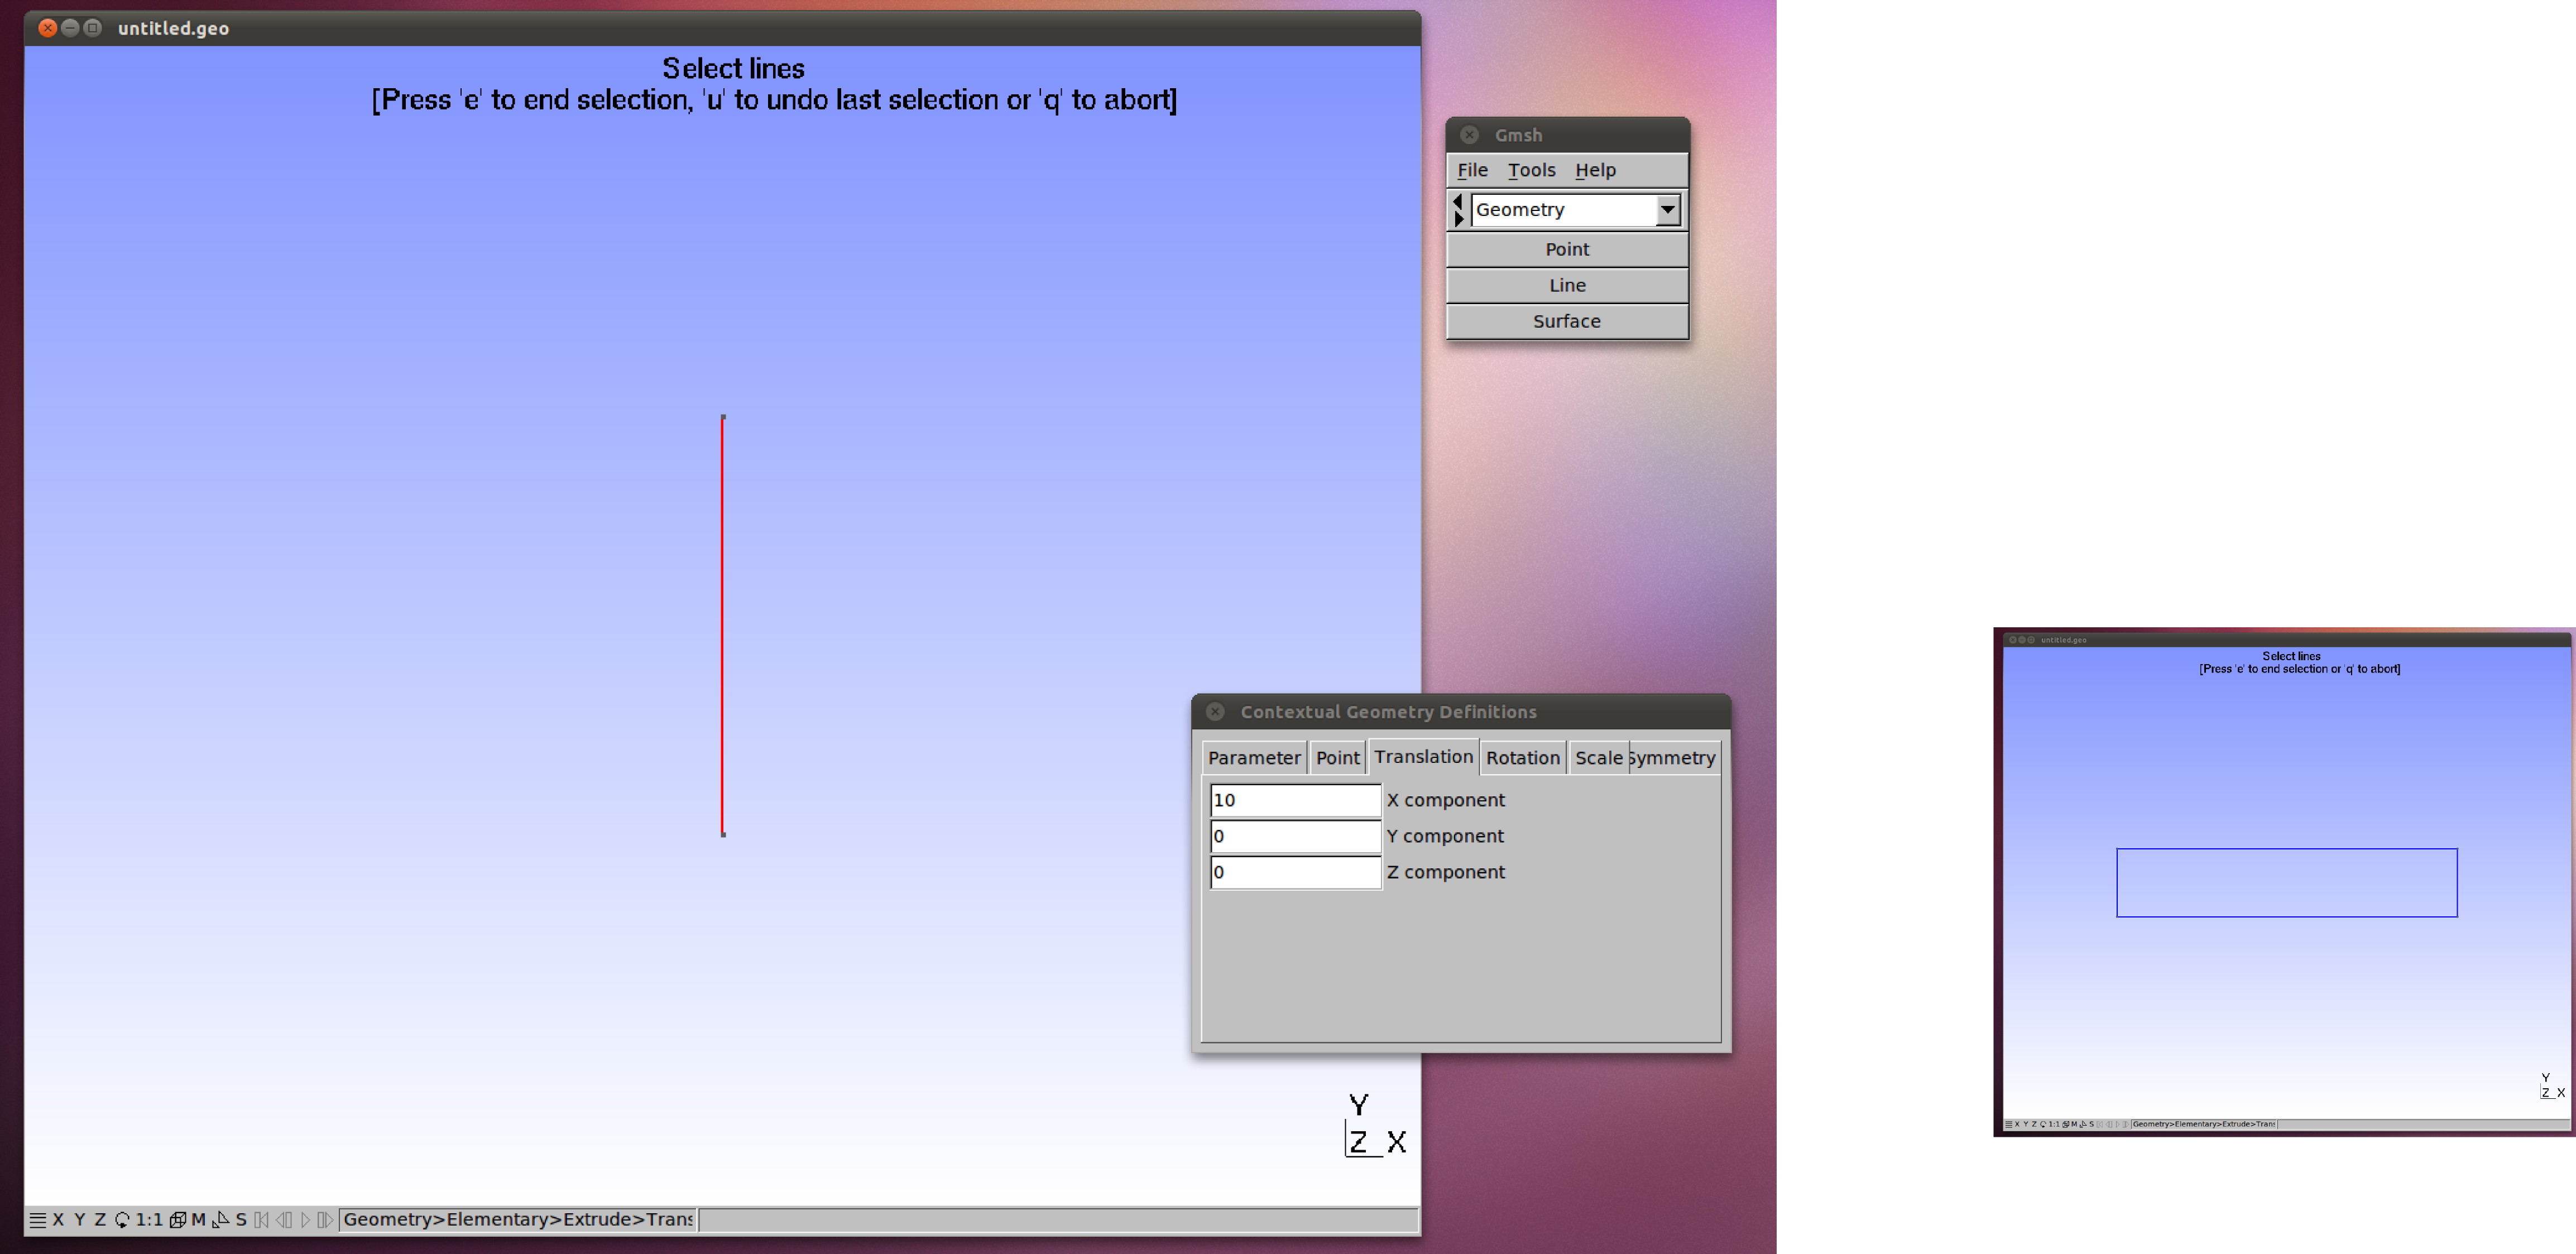
\includegraphics[width=1.0\textwidth]{../figures/extrusion.png}
  \caption{Extruding a line to form a rectangle.}
  \label{fig:extrusion}
\end{figure}
\par
%The following was not strictly necessary and was commented out. However it is not deleted, as it may
%be re-instated in a future version.
%The extrusion also defines a surface, the following steps show how to edit some of the gmsh options, so
%as to make Gmsh to highlight plane surfaces:
%\begin{enumerate}
%  \item On the menu bar of menu window of Gmsh click on ``Tools'' and select ``Options'', as highlighted
%        in the right panel of figure \ref{fig:gmsh_basic_options}. The ``Options'' window will appear.
%  \item In the Options window, select  the ``Visibility'' tab. On the side list select ``Geometry'' and
%        if not already activated, activate ``Surfaces'' (see left panel of figure
%        \ref{fig:gmsh_basic_options}).
%\end{enumerate}
%The interior of the square should now be marked with a gray, chain line as shown in
%figure \ref{fig:gmsh_basic_options}
%\begin{figure}[htbp]
% \centering
%  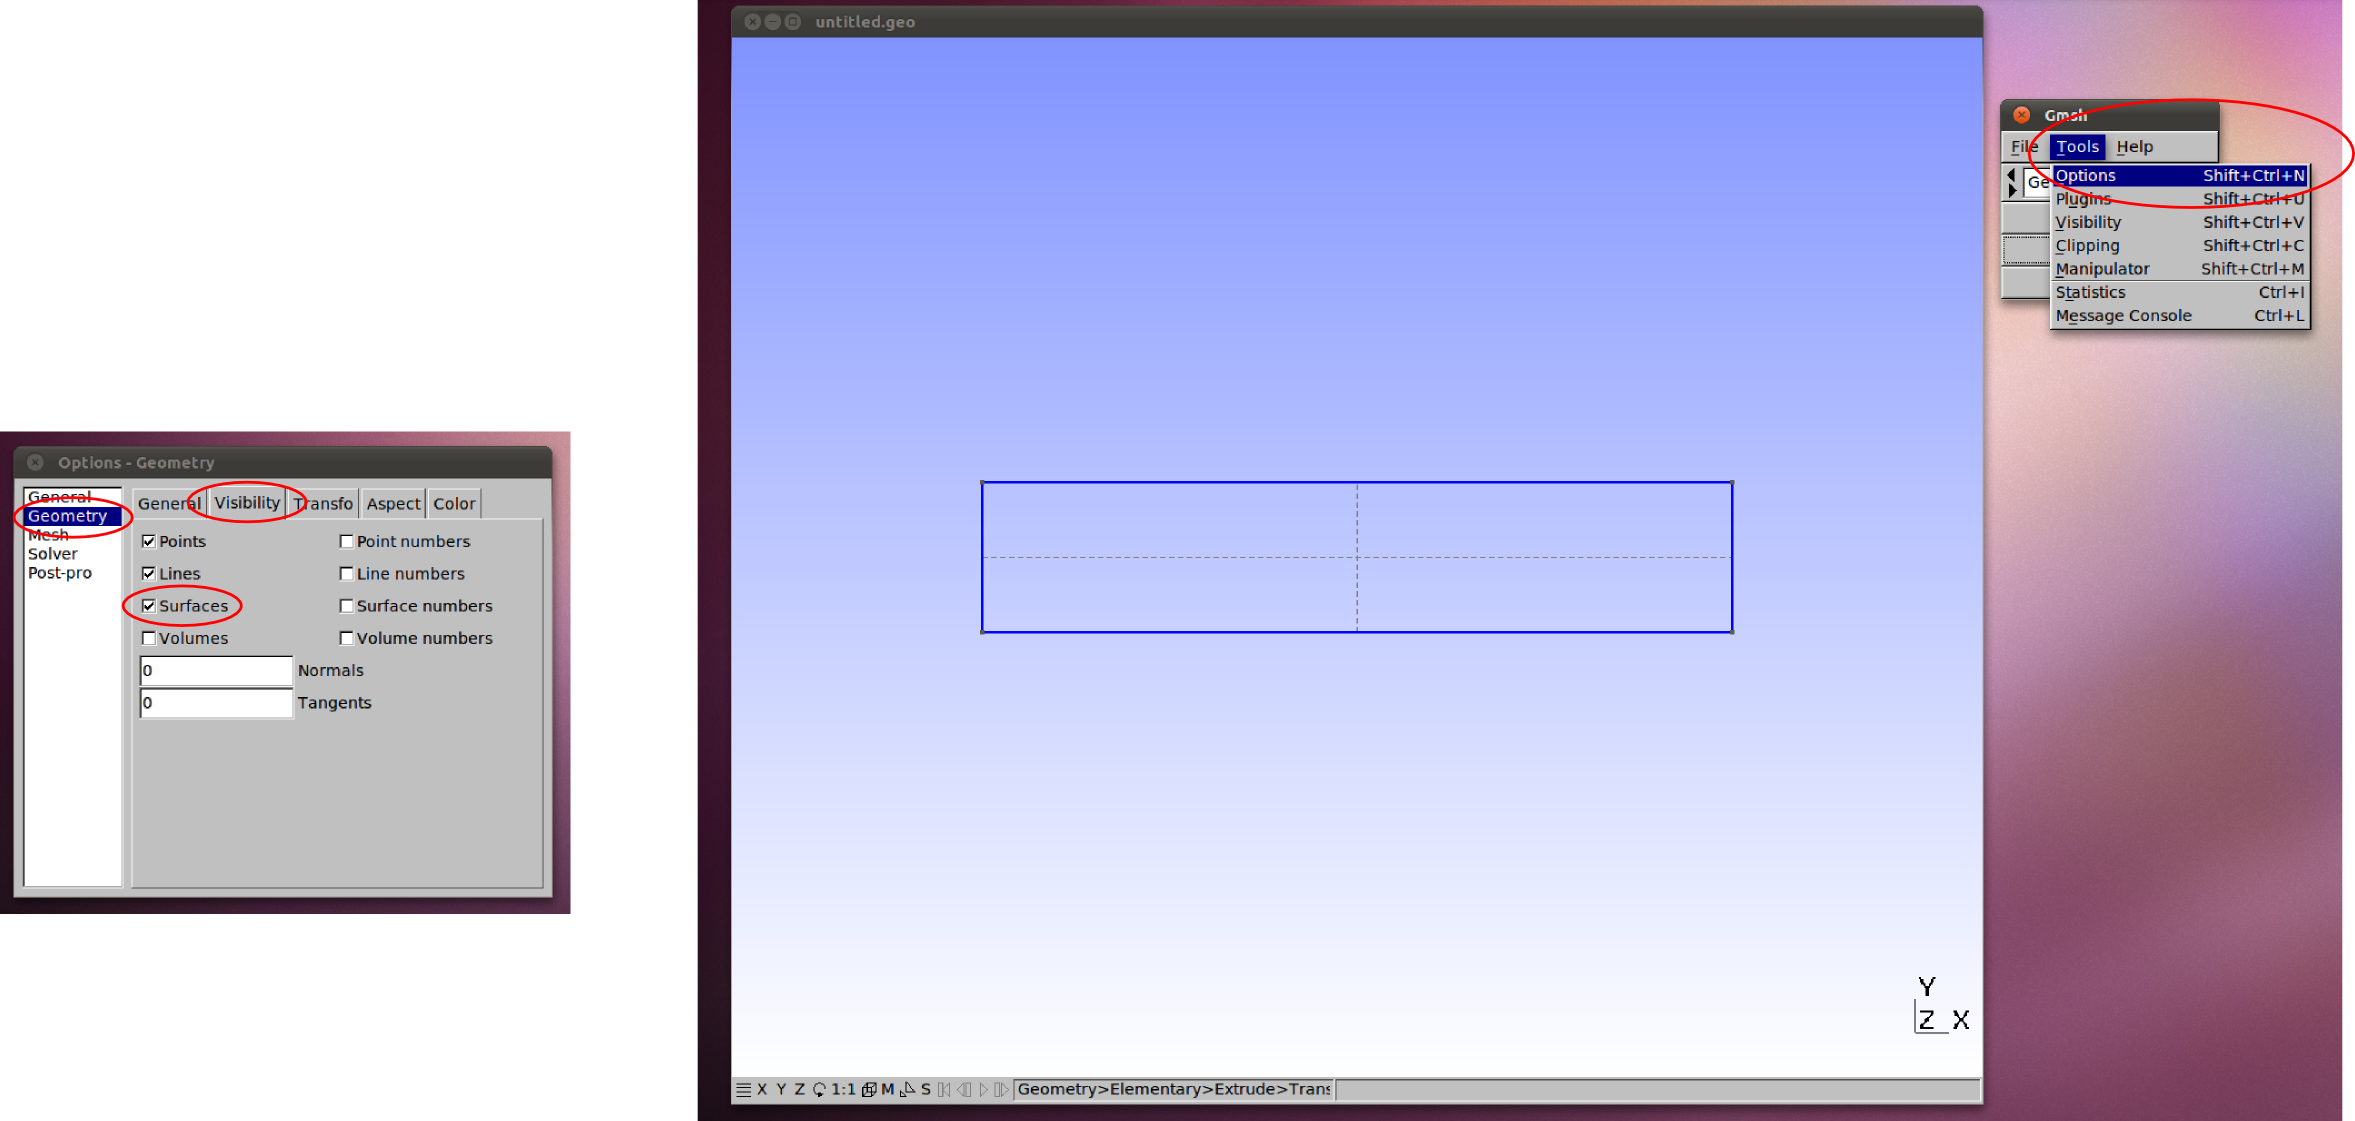
\includegraphics[width=1.0\textwidth]{../figures/gmsh_basic_options.png}
%  \caption{Changing the Gmsh options to highlight defined surfaces on the graphic window.}
%  \label{fig:gmsh_basic_options}
%\end{figure}

\subsection{Physical groups: boundaries and regions}
\label{ssect:2d_physical_groups}
\par
In order to apply boundary conditions it is necessary to specify ``Physical groups'' to which the boundaries belong. Since Gmsh will only export to a file those elements which are associated with a physical entity, it is also necessary to identify the interior of the domain with a physical group. Declare a physical surface over the interior of the rectangle as follows:
\begin{enumerate}
  \item Go to the top-most level of the Geometry module in the menu window.
  \item Click on \lstinline{Geometry > Physical group > Add > Surface}.
  \item Gmsh will highlight any surfaces with grey broken lines, see figure \ref{fig:shot15}
        for example.
  \item Select the plain-surface created in section \ref{ssect:setting_up_geometry}, by clicking on the
        broken grey line.
  \item Press ``e'' on your keyboard to end the selection, and then ``q''.
\end{enumerate}
Then declare physical lines from the edges of the rectangle as follows:
\begin{enumerate}
  \item On the menu window of Gmsh click on ``Line'', pick the top side of the rectangle and
        press ``e'' on your keyboard to end the selection.
  \item Pick the top side and the bottom side of the rectangle and press ``e'' on your keyboard to
        end the selection.
  \item On the menu window of Gmsh click on ``Line'', pick the left-hand side of the rectangle and
  \item Repeat the above step, selecting the right-hand-side of the rectangle.
  \item press ``q'' to exit the selection mode.
\end{enumerate}

\subsection{Final customisation of the geometry}
\label{ssect:2d_geo_fine_tuning}
\par
So far, we have been using the graphical user interface to create a simple geometry. we will now
use a less-graphical oriented approach to adjust some important details. At the beginning of the
section Gmsh was invoked using file \lstinline{channel.geo}. The file \lstinline{channel.geo}
 includes a set of declarations that allow Gmsh to reconstruct the geometry, effectively allowing the user
to ``save'' the geometry. Since the \lstinline{channel.geo} file is an ASCII file, any text editor can be
used to edit it, however, we will here use the text editor invoked by Gmsh itself:
\begin{enumerate}
  \item Go to the top-most level of the geometry module in the Gmsh menu window.
  \item Click on \lstinline{Edit}, a text editor instance (usually emacs) will open the file
        \lstinline{channel.geo}, as shown in figure \ref{fig:shot15}.
\end{enumerate}

\begin{figure}[htbp]
 \centering
  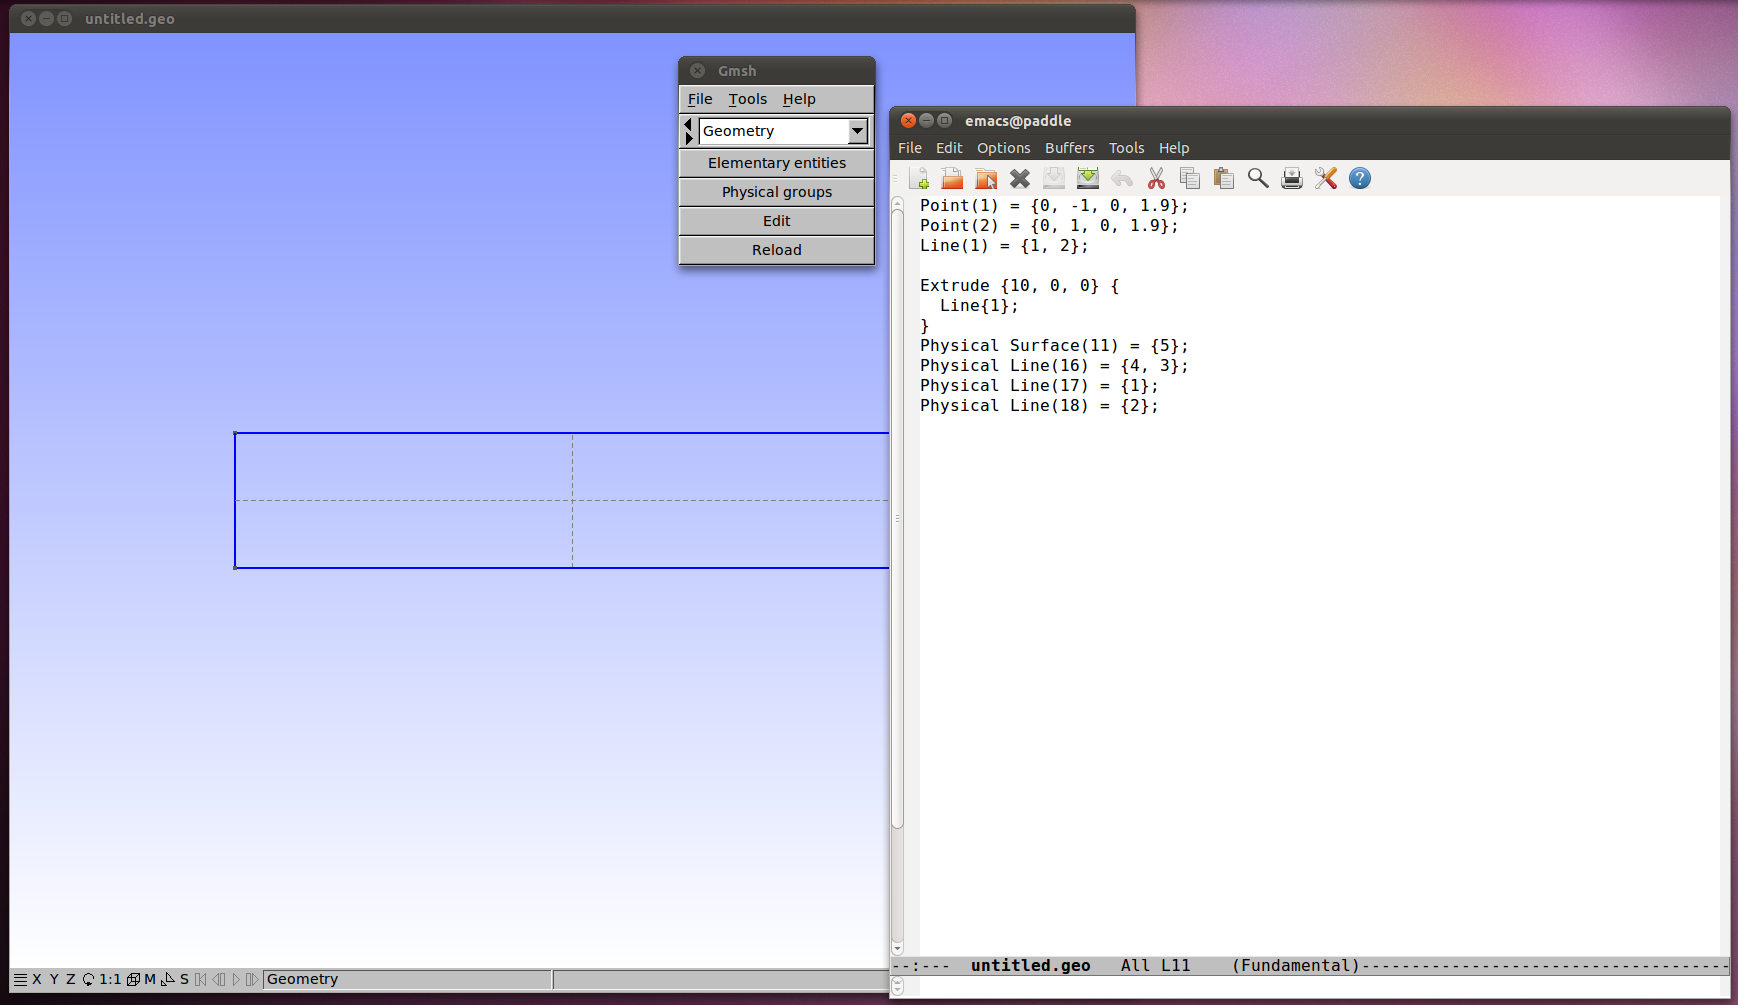
\includegraphics[width=1.0\textwidth]{../figures/shot15}
  \caption{The Gmsh windows with the text editor invoked on \lstinline{channel.geo}}
  \label{fig:shot15}
\end{figure}
\par
The file contents should be identical to the left hand-side of the listing below. The numbers present
on the left hand-side of the listings are added here for ease of reference. The \lstinline{.geo} files
are script files containing comments and expressions. Expressions can be further classified into 
string-expressions, floating-point expressions Loops \& Conditionals as well as other categories,
listing the categories is beyond the scope of this tutorial (however, the interested reader can find
the full documentation at \url{http://geuz.org/gmsh/doc/texinfo/gmsh.html#General-tools}). The expressions
of interest to this tutorial are commands that define geometrical objects. So, before the reader proceeds
with editing the file contents, we briefly describe the commands and the syntax of comments.
\begin{itemize}
  \item Lines preceded by \verb$//$ are comment lines and are ignored by Gmsh as it reads the file.
        Also any part of a script file between \verb$/*$ and \verb$*/$ is treated as a comment.
  \item Commands must terminate with \lstinline{;}, otherwise Gmsh assumes that the command is
        continued in the line below (see lines $5$ and $6$).\footnote{Also note that at the end of line
        $7$ a semi-colon should be present. Currently, its absence does not seem to affect Gmsh.}
  \item Commands such as those in line $1$, clearly create a point, and:
  \begin{itemize}
    \item Assign the point-ID in the round brackets on the left-hand-side of the expression to the
          point with coordinates specified by the first three numbers in the braces.
    \item Assign the fourth number in the braces as characteristic mesh size.
  \end{itemize}
  \item Commands such as those in line $3$, clearly create a line segment, and:
  \begin{itemize}
    \item Assign the line-ID in the round brackets on the left-hand-side of the expression to the
          line with endpoint specified by the point-IDs in the braces.
  \end{itemize}
  \item The extrusion command in line $5$ created the three remaining lines of the rectangle, as well
        as the plane surface
\end{itemize}

Edit the file, so as to match the right hand side listing.\\
\begin{minipage}[t]{0.48\textwidth}
\begin{center}
\lstinline+channel.geo+ file as produced by
GUI.
\end{center}
\lstset{numbers=left}
\begin{lstlisting}
Point(1) = {0, -1, 0, 1.9};
Point(2) = {0, 1, 0, 1.9};
Line(1) = {1, 2};

Extrude {10, 0, 0} {
  Line{1};
}
Physical Surface(11) = {5};
Physical Line(16) = {4, 3};
Physical Line(17) = {1};
Physical Line(18) = {2};
\end{lstlisting}
\lstset{numbers=none}
\end{minipage}
\hfill
\begin{minipage}[t]{0.48\textwidth}
\begin{center}
\lstinline+channel.geo+ file after
fine-tuning.
\end{center}
\lstset{numbers=left}
\begin{lstlisting}
Point (1) = {0, -1, 0, 1.9};
Point (2) = {0, 1, 0, 1.9};
Line (1) = {1, 2};

Extrude {10, 0, 0} {
  Line{1};Layers{20};
}

// Volume number for whole domain.
Physical Surface (1) = {5};
// Top and bottom of the box.
Physical Line(333) = {3,4};
// Left wall
Physical Line(666) = {1};
// Right wall
Physical Line(444) = {2};
\end{lstlisting}
\lstset{numbers=none}
\end{minipage}\\
In particular the following changes should be made:
\begin{enumerate}
  \item Append \verb$Layers{20};$ to line $6$. This instructs Gmsh to organise the mesh in $20$
        layers, normal to the extrusion direction.
  \item In line $9$ change \lstinline{Physical Line(16)} to \lstinline{Physical Line(333)}
  \item In line $10$ change \lstinline{Physical Line(17)} to \lstinline{Physical Line(666)}
  \item In line $11$ change \lstinline{Physical Line(18)} to \lstinline{Physical Line(444)}
  \item Insert comment-lines to match the left-hand-side listing above.
\end{enumerate}
Save the file and close the editor window. Click on \lstinline+Reload+ in the Gmsh menu window, Gmsh needs to read the updated file. You are now ready to generate a mesh.

\subsection{Producing a mesh}
\label{ssect:2d_producing_a_mesh}
\par
For the present example, generating a mesh once the geometry is properly defined is very simple:
\begin{enumerate}
  \item On the Gmsh menu window go to the mesh module (or press the ``m'' key).
  \item Click on ``2D''. A mesh should appear inside the rectangle, as shown in figure \ref{fig:shot16}.
  \item Save the mesh: Click on ``File'', then on ``Save mesh'' on the drop-down menu. The mesh is
        now saved in a file called \lstinline{channel.msh}
\end{enumerate}
\begin{figure}[htbp]
 \centering
  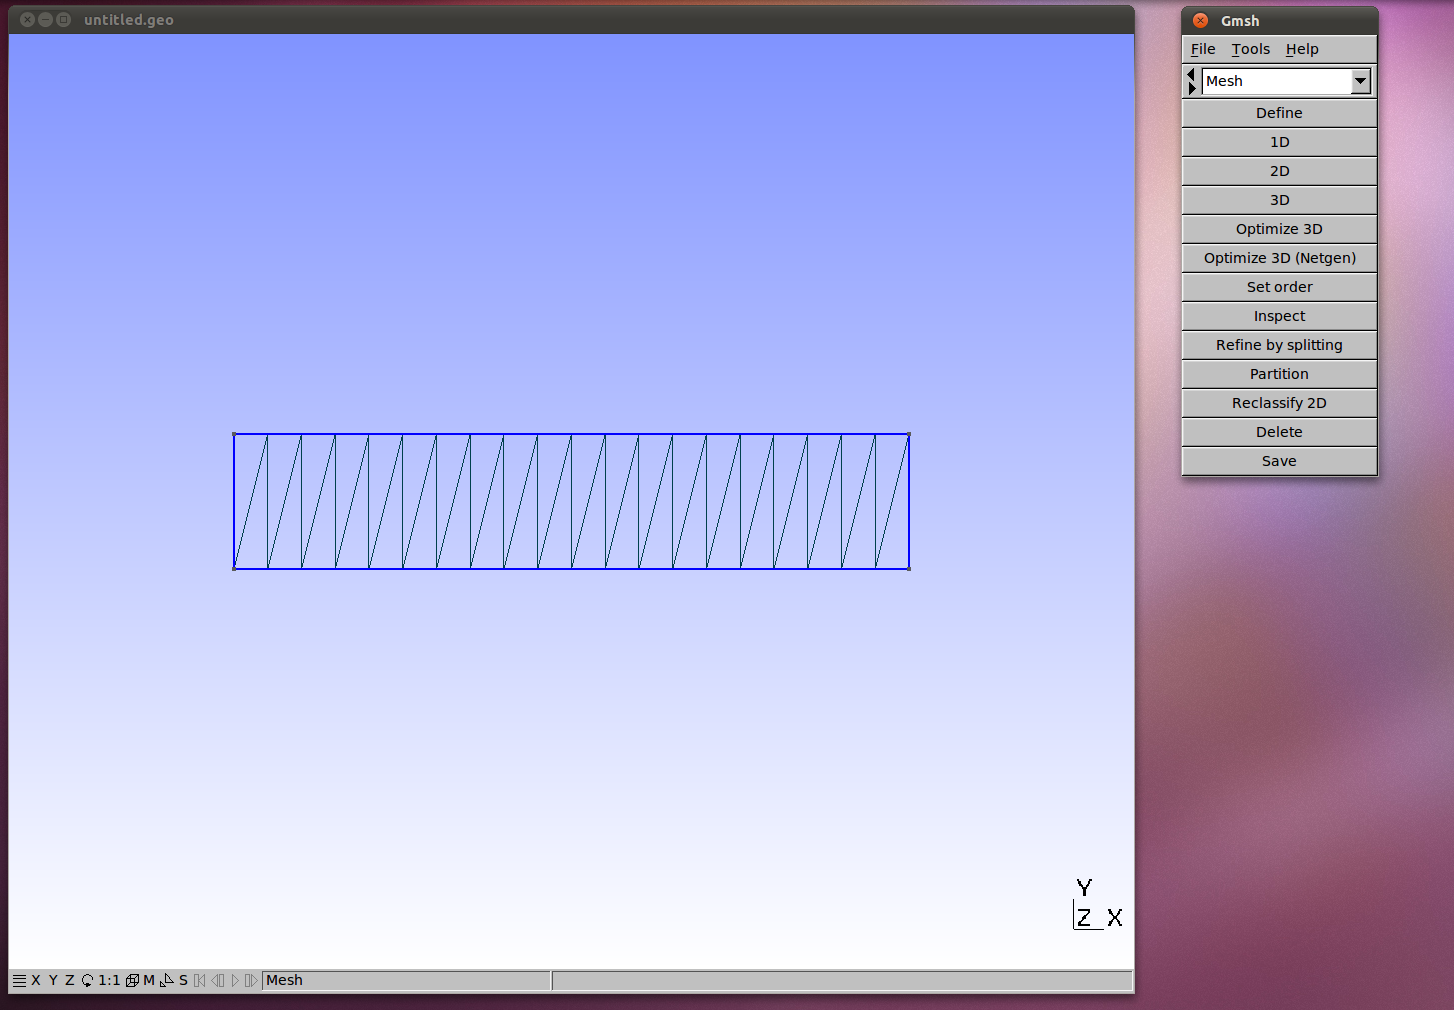
\includegraphics[width=1.0\textwidth]{../figures/shot16}
  \caption{The Gmsh windows showing the mesh.}
  \label{fig:shot16}
\end{figure}


\section{A three-dimensional, structured mesh example}
\label{sect:three_dimensional_example}
\par
The reader should be familiar with the geometry they will be creating in this section; the annulus
the reader opened and meshed in section \ref{ssect:basic_interaction_gmsh_gui} is the geometry
we will now create. The mesh however, will be of higher resolution. The following steps will be
undertaken, also outlined in figure \ref{fig:annulus_schematic}:
\begin{enumerate}
  \item Create the geometry using the Gmsh GUI:
  \begin{enumerate}
    \item A rectangle will be formed using a procedure similar to section
             \ref{sect:two_dimensional_example}. This rectangle represents a radial plane through the
             annulus, for example the plane outlined in red broken lines in the left panel of figure
             \ref{fig:annulus_schematic}.
    \item The plane will then be extruded-rotated in order to form a quadrant of the annulus, as
             shown in the right panel of figure \ref{fig:annulus_schematic}.
    \item The above step is then repeated, as indicated by the arrows in the top of the annulus on
             the left panel of figure \ref{fig:annulus_schematic}, until the complete annulus is formed
  \end{enumerate}
  \item Define physical groups.
  \item Customise the geometry by editing the geometry script file.
  \item Produce a mesh.
\end{enumerate}
\begin{figure}[htbp]
 \centering
  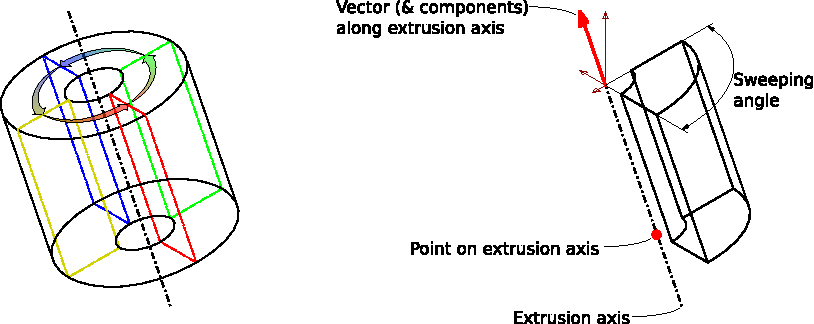
\includegraphics[width=1.0\textwidth]{../figures/annulus.pdf}
  \caption{Schematic of forming an annulus with extrusions}
  \label{fig:annulus_schematic}
\end{figure}

\subsection{Creating the geometry: Forming an annulus with extrusions}
\label{ssect:annulus_via_extrusions}
\par
Start Gmsh, at the command line using file \lstinline+annulus.geo+ to store the script. Create the three
points at the coordinates shown in table \ref{table:annulus_starting_points} below. The points should
lie on a line along the $x$-direction and form a radial line across the annulus. Create two lines: the
first line connecting point $1$ to point $2$ and the second
line connecting the point $2$ to point $3$. Then, extrude the lines to create surfaces
(extrude-translate, see figures \ref{fig:gmsh_extrusion} and \ref{fig:extrusion}), translating
by $(x,y,z)=(0.0, 0.0, 14.0)$. Note that both lines should be selected during the extrusion step.
Finally, change the view-point, so that you can see the rectangles just created, you should have
something similar to the graphic window in figure \ref{fig:extruding_red_plane}, corresponding to
the plane highlighted by the red broken line in the left panel of figure \ref{fig:annulus_schematic}
\begin{table}[htdp]
  \caption{Coordinates and mesh size at the starting points when making an annulus.}
  \centering
  \begin{tabular}{|r|c|c|c|c|}\hline
  point ID & $x$-coord. & $y$-coord. & $z$-coord. & Mesh element size \\ \hline
  $1$      & $2.5$      & $0.0$      & $0.0$      & $0.1$ \\ \hline
  $2$      & $5.25$     & $0.0$      & $0.0$      & $1.0$ \\ \hline
  $3$      & $8.0$      & $0.0$      & $0.0$      & $0.1$ \\ \hline
  \end{tabular}
  \label{table:annulus_starting_points}
\end{table}
\begin{figure}[htbp]
 \centering
  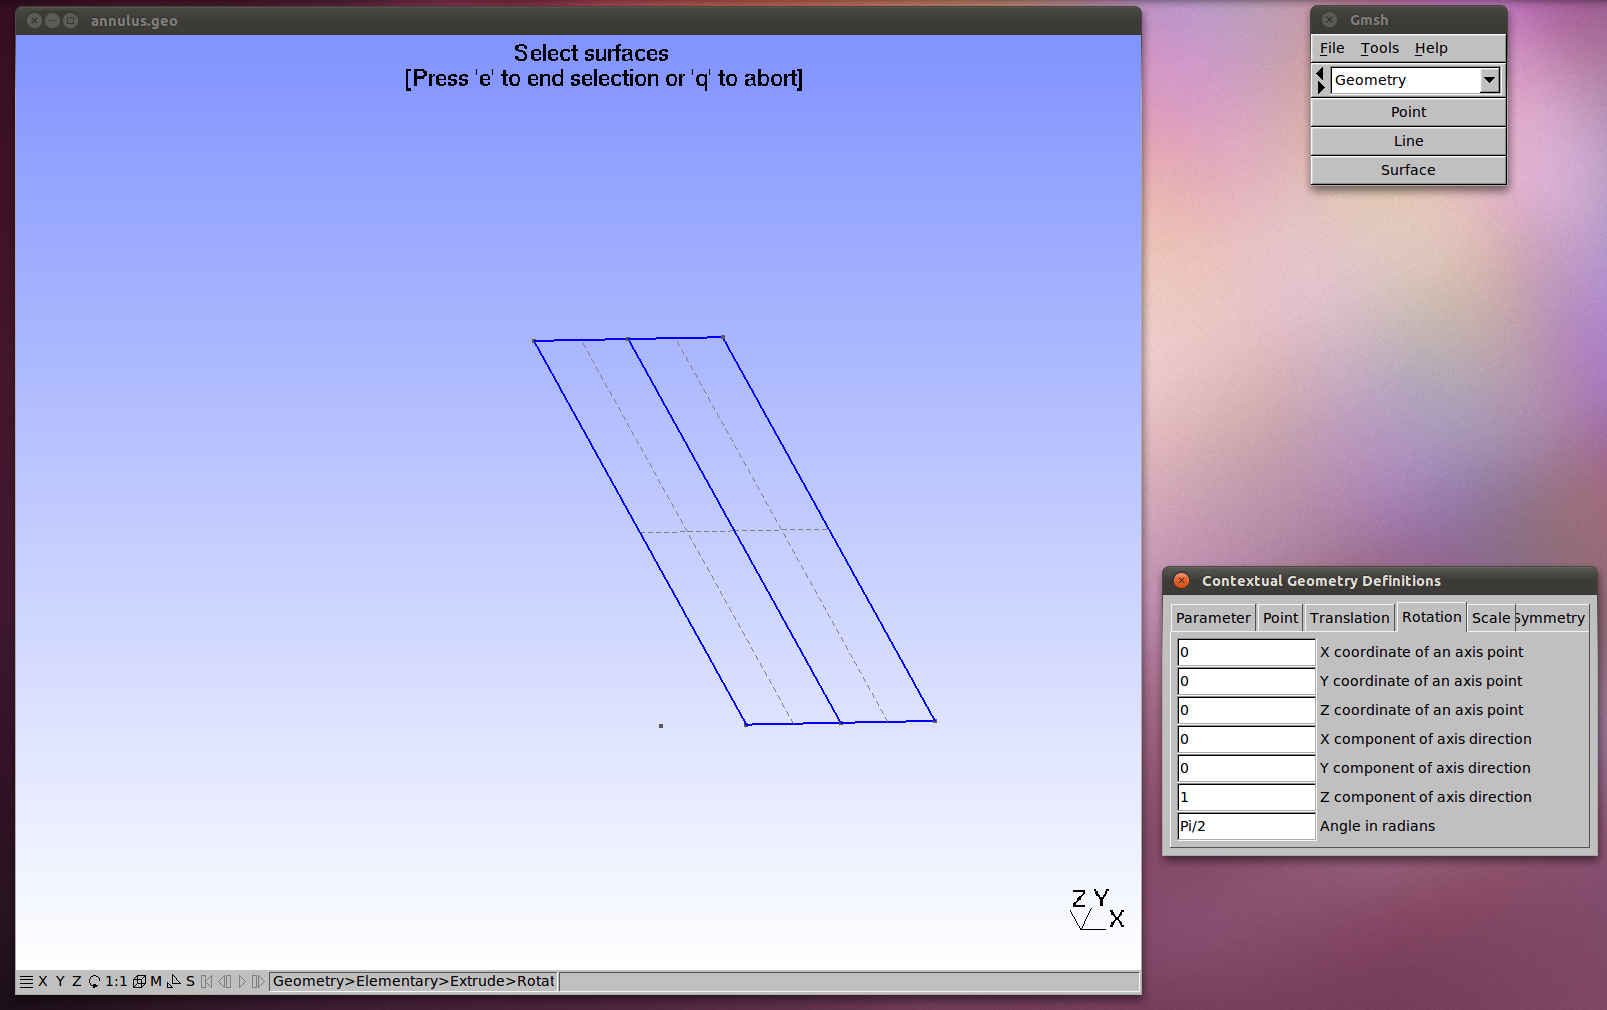
\includegraphics[width=1.0\textwidth]{../figures/shot17.png}
  \caption{The Graphic, Menu and Contextual Geometry Definitions windows during an 
                extrusion-via-revolution step.}
  \label{fig:extruding_red_plane}
\end{figure}
\par
The next step is to extrude-rotate the rectangular surface in order to create the annulus.
\begin{enumerate}
  \item Go to the top-most level of the Geometry module in the Gmsh menu window.
  \item Click on \lstinline+Elementary entities > Extrude > Rotate > Surface+. The
        Contextual Geometry Definitions window will appear, on the Rotation tab. Also the surfaces will
        now be highlighted on the graphic window, as shown in the graphic window of figure
        \ref{fig:extruding_red_plane}. The Contextual Geometry Definitions window is used to define
        the axis of revolution and the sweeping angle. The axis of revolution is defined by specifying any
        point on it and the components of a vector parallel to the axis. (\eg the red point and red vector
        components in the right panel of figure \ref{fig:annulus_schematic}). In addition, the sweeping angle
        must be specified in radians, in the anti-clockwise sense.
  \item Change the parameters in the Contextual Definitions window to the following:
  \begin{itemize}
    \item X coordinate of an axis point: $0$
    \item Y coordinate of an axis point: $0$
    \item Z coordinate of an axis point: $0$
    \item X component  of axis direction: $0$
    \item Y component  of axis direction: $0$
    \item Z component  of axis direction: $1$
    \item Angle in radians: Pi/$2$
  \end{itemize}
  \item Pick both surfaces on the graphic window and press ``e''. A quarter of the annulus should have been
        formed in the graphic window, as shown in left panel of figure \ref{fig:completing_the_annulus}. 
        Without changing the parameters in the Contextual Geometry Definitions
        window, pick the newly formed surfaces normal to the $x$-axis (surface demarcated in green in figure
        \ref{fig:annulus_schematic}) and press the ``e'' key, to form half the annulus. Repeat the
        procedure to form the complete annulus, shown in the right panel of figure
        \ref{fig:completing_the_annulus}. 
\end{enumerate}
\begin{figure}[htbp]
 \centering
  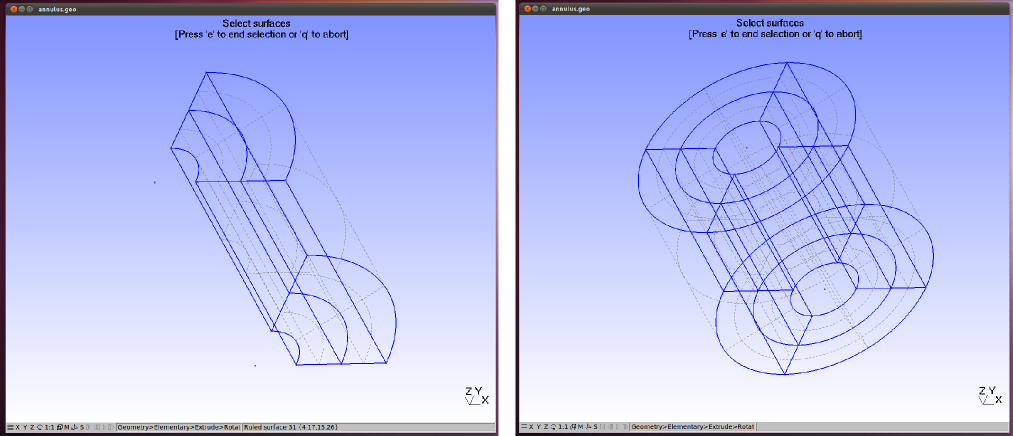
\includegraphics[width=1\textwidth]{../figures/completing_the_annulus.png}
  \caption{The Gmsh window showing a quadrant (left panel) and the complete annulus (right panel).}
  \label{fig:completing_the_annulus}
\end{figure}

\subsection{Physical groups}
\label{ssect:3d_physical_groups}
\par
As in the previous section physical surfaces and volumes must be specified, start by specifying physical
surfaces:
\begin{enumerate}
  \item Go to the top-most level of the Geometry module in the Gmsh menu window.
  \item Click on \lstinline+Physical groups > Add > Surface+. Select the $8$ surfaces comprising the
        top of the annulus and press ``e''. Obviously you can pan, zoom and change your viewpoint
        to make selection easier. Press ``u'' to undo your last selection as hinted on the graphic
        window, if a wrong choice is made.
  \item Repeat for the bottom of the annulus, the inner wall, and the outer wall (in that order).
  \item Press ``q'' to abort the selection mode and end the command.
\end{enumerate}
Then specify physical volumes:
\begin{enumerate}
  \item Click on \lstinline+Volume+, on the Gmsh menu window. Volumes created by extrusions will
           be indicated by yellow spherical markers, one per volume entity.
  \item Pick all of the spherical markers. Once picked, a volume marker is highlighted in red.
  \item Press ``e'' to end the selection.
\end{enumerate}

\subsection{Final customisation of the script and mesh production}
\label{ssect:3d_geo_fine_tuning}
\par
At this point, a mesh can be produced, suitable for Fluidity simulations. The mesh will be unstructured
and it is left as an exercise to the reader to mesh the geometry. Should you choose to mesh the geometry at
this point, then once finished you must go to the top-most level of the Geometry module and click on
\lstinline+Reload+ to re-join us for this tutorial. The script is now modified to make Gmsh produce a
structured mesh:
\begin{enumerate}
  \item Open the script in a text editor.
  \item The script should be \emph{similar} to the first listing below.
  \item Edit the script to make it similar to the second listing below, and save it. You only
        have to append the \lstinline+Layers{};+ statements and insert the comments.
  \item Go to the top-most level of the Geometry module in the Gmsh menu window. and click
        \lstinline+Reload+.
\end{enumerate}
\lstinline+annulus.geo+ file as produced by
GUI.
\lstset{numbers=left}
\begin{lstlisting}
Point(1) = {2.5, 0, 0, 0.1};
Point(2) = {5.25, 0, 0, 1.0};
Point(3) = {8, 0, 0, 0.1};
Line(1) = {1, 2};
Line(2) = {2, 3};
Extrude {0, 0, 14} {
  Line{1, 2};
}
Extrude {{0, 0, 1}, {0, 0, 0}, Pi/2} {
  Surface{6, 10};
}
Extrude {{0, 0, 1}, {0, 0, 0}, Pi/2} {
  Surface{32, 54};
}
Extrude {{0, 0, 1}, {0, 0, 0}, Pi/2} {
  Surface{98, 76};
}
Extrude {{0, 0, 1}, {0, 0, 0}, Pi/2} {
  Surface{120, 142};
}
Physical Surface(185) = {93, 49, 159, 115, 71, 27, 180, 137};
Physical Surface(186) = {107, 151, 41, 85, 63, 19, 172, 129};
Physical Surface(187) = {141, 184, 31, 75};
Physical Surface(188) = {89, 111, 155, 45};
Physical Volume(189) = {4, 3, 1, 2, 8, 7, 5, 6};
\end{lstlisting}
\lstset{numbers=none}
\lstinline+annulus.geo+ script after editing.
\lstset{numbers=left}
\begin{lstlisting}
Point(1) = {2.5, 0, 0, 0.1};
Point(2) = {5.25, 0, 0, 1.0};
Point(3) = {8, 0, 0, 0.1};
Line(1) = {1, 2};
Line(2) = {2, 3};
Extrude {0, 0, 14} {
  Line{1, 2};Layers{25};
}
Extrude {{0, 0, 1}, {0, 0, 0}, Pi/2} {
  Surface{6, 10};Layers{30};
}
Extrude {{0, 0, 1}, {0, 0, 0}, Pi/2} {
  Surface{32, 54};Layers{30};
}
Extrude {{0, 0, 1}, {0, 0, 0}, Pi/2} {
  Surface{98, 76};Layers{30};
}
Extrude {{0, 0, 1}, {0, 0, 0}, Pi/2} {
  Surface{120, 142};Layers{30};
}
// Top
Physical Surface(185) = {93, 49, 159, 115, 71, 27, 180, 137};
// Bottom
Physical Surface(186) = {107, 151, 41, 85, 63, 19, 172, 129};
// Inner wall
Physical Surface(187) = {141, 184, 31, 75};
// Outer wall
Physical Surface(188) = {89, 111, 155, 45};
Physical Volume(189) = {4, 3, 1, 2, 8, 7, 5, 6};
\end{lstlisting}
\lstset{numbers=none}
\par
To mesh the annulus, go to the top-most level of the Mesh module and click ``3D'' on the Gmsh menu
window.Notice the gradation in cell size towards the wall, affected by a different characteristic mesh size in
Point $2$, see table \ref{table:annulus_starting_points} and the listings above.


\section{Mesh generation on spherical manifolds}
\label{sect:spherical_manifolds}
\par

In this example, we generate a mesh of a section of the ocean on the surface of a sphere (the Earth). Within just a few steps, we will be able to produce a mesh
similar to figure~\ref{fig:sphericalpatch}.

\begin{figure}[htbp]
 \centering
  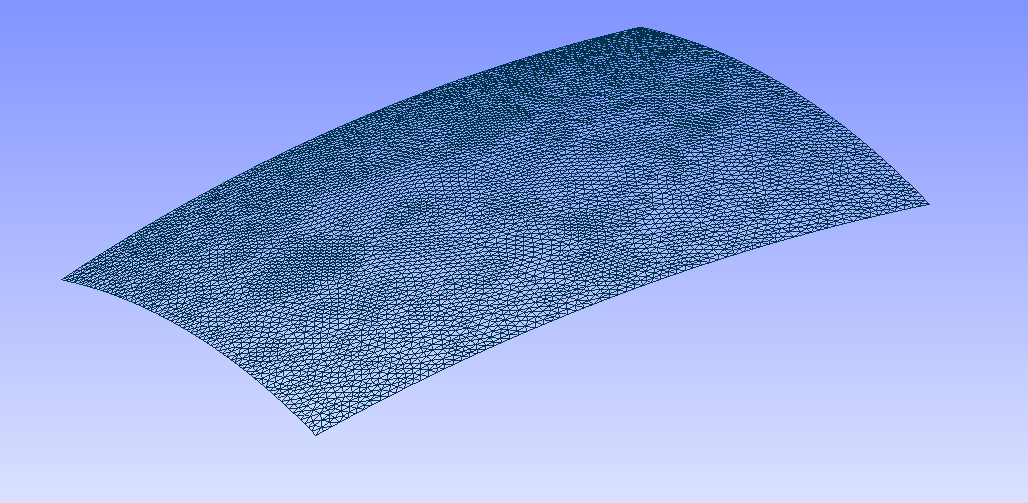
\includegraphics[width=1.0\textwidth]{../figures/sphericalpatch}
  \caption{A 2--D manifold in 3--D space.}
  \label{fig:sphericalpatch}
\end{figure}

We will make primary use of the Gmsh scripting language and resort to the graphical user interface only to ensure that we are progressing correctly. We will be saving the script with the .geo extension, which Gmsh recognises as its own. To generate a file manifold.geo, we may issue:
\begin{lstlisting}
gedit manifold.geo
\end{lstlisting}
which opens the gedit text editor and generates the manifold.geo file.

In this chapter you will learn how to:
\begin{enumerate}
\item Define points on the sphere (section~\ref{sect:definepointsmanifold}).
\item Connect the points with lines (section~\ref{sect:definelinesmanifold}).
\item Define physical surfaces and generate meshes on the sphere (section~\ref{sect:meshgenerationmanifold}).
\end{enumerate}

First, however, we will be introducing the process of stereographic projection (section~\ref{sect:stereoprojection}). This is important because we need to define points on the projected plane before Gmsh automatically maps them back to the sphere.

\subsection{Background: Stereographic projection}
\label{sect:stereoprojection}
A stereographic projection, $\sigma$, maps all points (apart from one, the \emph{North Pole}) of an $n$--dimensional unit sphere, $S^n \in  R^{n+1}$, to an $n$--dimensional plane:
%%
\begin{align}
\sigma : S^n \rightarrow R^n
\end{align}
%%
Figure~\ref{fig:2dstereoprojection} illustrates a two-dimensional sphere being projected onto a line.

\begin{figure}[htbp]
 \centering
  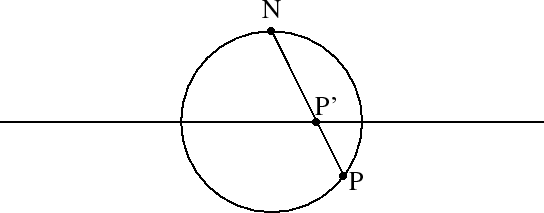
\includegraphics[width=0.9\textwidth]{../figures/2dstereoprojection}
  \caption{2--D stereographic projection. Point N indicates the North Pole. Point P` is the projection of Point P.}
  \label{fig:2dstereoprojection}
\end{figure}

%Don't forget to cite the Wolfram Alpha website.

\subsection{Defining Points}
\label{sect:definepointsmanifold}
Gmsh has the capability of plotting points on the sphere. To the user`s convenience, only the projections of these points need to be defined. Prior to these points, however, two special points are required:
\begin{enumerate}
  \item The center of the sphere.
  \item The \emph{North Pole}.
\end{enumerate}

To start our example, open a plain file and begin by defining the special points described:
\begin{lstlisting}
Point(1) = {0.0,0.0,0.0};         //The center of the sphere
Point(2) = {0.0,0.0,6.37101e+06}; //The North Pole
\end{lstlisting}
We then need to inform Gmsh that any further points defined, will be on the sphere. So we issue the following statement:
\begin{lstlisting}
PolarSphere(1) = {1,2}; //Sphere with center at Point(1)
                        //and North Pole at Point(2).
\end{lstlisting}

We now proceed by defining the remaining points, with coordinates on the 2--D plane. In this example, we will create a domain that spans from +10 to +30 degrees in longitude and +5 to +25 in latitude.

\begin{lstlisting}
//Point 3: 10 lon 5 lat

//First we convert to radians
//and then to stereographic coordinates.
Point_lon_rad = (10)*(Pi/180);
Point_lat_rad = (5)*(Pi/180);
Point_3_stereographic_x = -Cos(Fabs(Point_lon_rad))*Cos(Fabs(Point_lat_rad))/
    ( 1 + Sin(Fabs(Point_lat_rad)) );
Point_3_stereographic_y = Cos(Fabs(Point_lat_rad))*Sin(Fabs(Point_lon_rad))/
    ( 1 + Sin(Fabs(Point_latx_rad)) );

//Now we define the point
Point(3) = {Point_stereographic_x, Point_stereographic_y,0};
\end{lstlisting}

We must repeat the process for the remaining three points:
\begin{itemize}
\item[-] Point 4: 10 lon 25 lat
\item[-] Point 5: 30 lon 25 lat
\item[-] Point 6: 30 lon 5 lat
\end{itemize}

After we have defined the center, north pole and 4 edges of our domain; it is sensible to open up the file in Gmsh to have a look at our progress. We first save the file and then open it in Gmsh by issuing the following command at the terminal:
\begin{lstlisting}
gmsh manifold.geo
\end{lstlisting}
The center and north pole should be visible, as well as the 4 points on the surface of the sphere, as in figure~\ref{fig:pointsdefinition}.

\begin{figure}[htbp]
 \centering
  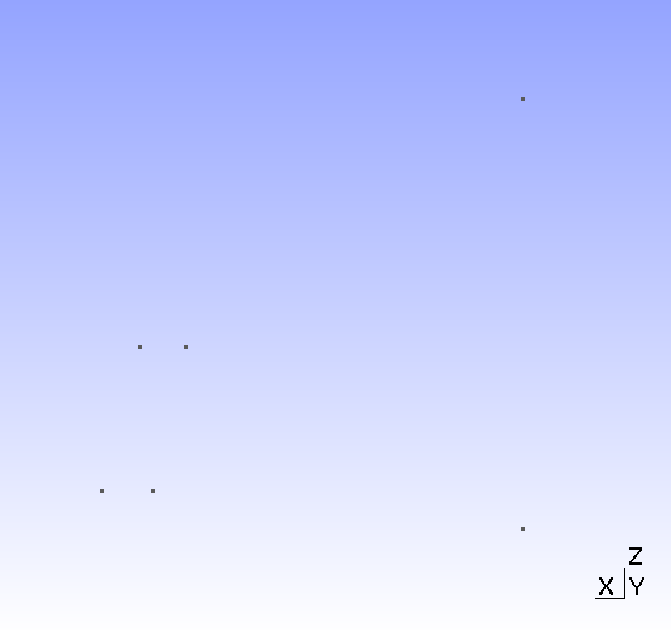
\includegraphics[width=0.9\textwidth]{../figures/pointsdefinition}
  \caption{The center of the sphere (below right), as well as the North pole (top right) and the four edges of the domain are visible in Gmsh. It is clear by looking at the coordinate system that the four points have been mapped from the 2--D plane.}
  \label{fig:pointsdefinition}
\end{figure}

\subsection{Defining zonal and meridional lines}
\label{sect:definelinesmanifold}
In stereographic projection of a 2--D sphere such as the Earth, lines of constant latitude are mapped to straight lines in a plane. Gmsh is therefore able to accurately interpolate meridional lines, given just two points. Lines of constant longitude however, are projected to circles in the plane. The arcs between these points are also approximated by straight lines in Gmsh so a poor result is obtained if the distance between the points is large.

To correct this problem, we break any zonal paths into smaller segments for which the straight line assumption is valid. We will be using the following function:
\begin{lstlisting}
Function DrawParallel
 alpha = parallelSectionStartingY/parallelSectionStartingX;
 parallelRadius = Sqrt(parallelSectionStartingX^2 + parallelSectionStartingY^2);
 deltaAlpha = (parallelSectionEndingY/parallelSectionEndingX - 
    parallelSectionStartingY/parallelSectionStartingX)/pointsOnParallel;
 For t In {1:pointsOnParallel}
  alpha += deltaAlpha;
  newParallelPointX = (parallelSectionStartingX/Fabs(parallelSectionStartingX))
     *parallelRadius/(Sqrt(alpha^2 + 1));
  newParallelPointY = newParallelPointX*alpha;
  newPointOnParallel = newp;
  Point(newPointOnParallel) = {newParallelPointX, newParallelPointY, 0};
 EndFor
 BSpline(newParallelID) = {firstPointOnParallel, newPointOnParallel-
     (pointsOnParallel-1):newPointOnParallel, lastPointOnParallel};
Return
\end{lstlisting}

The function we have just defined requires the following parameters to be set prior to being called:
\begin{itemize}
\item pointsOnParallel : The number of points to be defined between the two we have already defined.
\item parallelSectionStartingX : The first stereographic coordinate of the starting point. If we are drawing the southernmost zonal line, this will be the x-coordinate of the south-westernmost point (Point(3) in our case). The Y coordinate is also required in a respectively named parameter, as well as the X and Y coordinates of the ending point (south-easternmost point, Point(6)).
\item firstPointonParallel : In addition to its coordinates, the function needs to know the point number of the first and last points of the zonal line.
\item newParallelID : Finally, each line we draw needs a unique number.
\end{itemize}

We can now go ahead and plot the zonal lines by appending the following to our manifold.geo file:

\begin{lstlisting}
//Draw south-most parallel of the Domain. Point 3 to Point 6

//Assign parameters to variables and then call function DrawParallel,
pointsOnParallel = 200;
parallelSectionStartingX = Point_3_stereographic_x;
parallelSectionStartingY = Point_3_stereographic_y;
firstPointOnParallel = 3;
parallelSectionEndingX = Point_6_stereographic_x;
parallelSectionEndingY = Point_6_stereographic_y;
lastPointOnParallel = 6;
newParallelID = 1;
Call DrawParallel;
\end{lstlisting}

The meridional lines are much simpler, and can be drawn by simply specifying to Gmsh that we require a B-spline between the two points:

\begin{lstlisting}
//Draw western-most meridional
BSpline(3) = {3, 4};
//Draw eastern-most meridional
BSpline(4) = {5, 6};
\end{lstlisting}

Saving and opening the manifold.geo file in Gmsh should now look like what we see in figure~\ref{fig:linesdefinition}.

\begin{figure}[htbp]
 \centering
  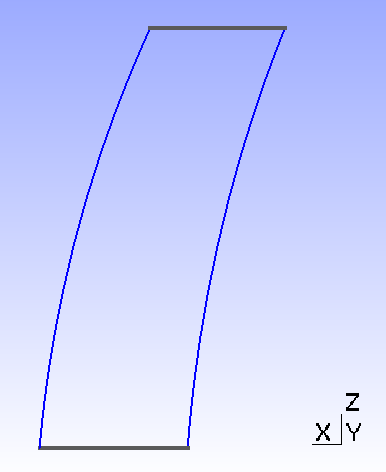
\includegraphics[width=0.7\textwidth]{../figures/linesdefinition}
  \caption{The points of figure~\ref{fig:pointsdefinition} have now been connected by lines. Note that zonal lines have had points defined along their path, as requested in the function we defined.}
  \label{fig:linesdefinition}
\end{figure}


\subsection{Mesh generation}
\label{sect:meshgenerationmanifold}
All that remains to generate the mesh is to specify the Physical surface and a Field to instruct Gmsh of the desired element length.

\begin{lstlisting}
//Define new line from previously generated lines that generates a loop.
Line Loop(6) = {3,2,4,-1};
Plane Surface(7) = {6}; //Surface from Loop
Physical Surface(8) = {7};

Field[50] = MathEval; //Generate Field
Field[50].F = "30000";
Background Field = 50;
\end{lstlisting}

The variable \lstinline{Field[50].F} should equal the desired element edge size. In our example, we set it equal to a constant \lstinline{30000} indicating we want a constant element edge size of $30km$. This value could have been any other mathematical expression to be evaluated by Gmsh.

We can now instruct Gmsh to mesh the defined domain by issuing the following command at the terminal:
\begin{lstlisting}
gmsh -3 manifold.geo
\end{lstlisting}
This will produce a file manifold.msh which can be opened in Gmsh. This will give you a mesh such as that shown in figure~\ref{fig:sphericalpatch}.

The full .geo file used in this example is given:

\lstinputlisting{../figures/spherical_manifold_example.txt}


\section{Ocean mesh generation}
\label{sect:ocean_mesh_generation}
In this section we briefly present the procedure of mesh generation on domains representative of realistic oceans, including shorelines. Clearly, the shorelines need to be extracted from a relevant source and be reconstructed in the Geometry module of Gmsh. For that purpose, Gmsh features the \emph{GSHHS plugin} \citep{lambrechts_et_al:2008}. As its name suggests, this plugin uses the \emph{Global Self-consistent, Hierarchical, High-resolution Shoreline Database}\footnote{available from \url{http://www.ngdc.noaa.gov/mgg/shorelines/gshhs.html}} \citep{wessel_smith:1996} as a source of shoreline contours. In specific, the plugin allows the user to select an area on the globe, and then generates a Gmsh geometry script fitting a spline to the shoreline points. The user can then draw open boundaries to form a closed domain. 
\par
The interested reader is deferred to \url{http://perso.uclouvain.be/jonathan.lambrechts/gmsh_ocean/} where screen-casts show how to use the plugin and generate meshes featuring higher resolution to towards the shoreline. However, the user can specify plugin options and then invoke plugins from within Gmsh scripts. Thus, a procedure where the user creates a series of scripts and semi-automates the procedure will be presented here in the near future.

%\par
%In this section we first show how to create geometries on a spherical manifold representative of shorelines. Then, combined with the methodology for drawing lines of constant longitude or constant latitude developed in the previous section, the reader will learn how to produce meshes on geometries representing realistic ocean domains.
%\par
%what is gshhs? how does one obtain it? Must give some configuration steps here
%\par
%What is the Gmsh GSHHS plugin? (no need for separate download, it comes with Gmsh!). Must give an overview of the plugin: its options and what they do.
%
%\subsection{Setting up the geometry}
%\label{ssect:setting_up}
%
%\subsubsection{Selecting the area on Earth to be meshed.}
%\par
%Show maps (reference Generic Mapping Tools), identify points, identify boxes, list point coordinates.
%
%\subsubsection{Some definitions}
%
%\subsubsection{Extracting the shoreline}
%
%\subsubsection{Drawing the open boundaries}
%
%\subsubsection{Specifying the mesh sizes}
%
%\subsection{Producing a mesh} 


%\section{Further reading}
\label{sect:additional_material}
give links to amcg wiki, gmsh web-site, usefull screen casts.



\addcontentsline{toc}{section}{References}
\bibliographystyle{apalike}
\bibliography{biblio.bib}
\end{document}
